%
% chapter.tex
%
% (c) 2023 Prof Dr Andreas Müller
%
\chapter{Extremalprobleme für Funktionen mehrere Variablen
\label{buch:chapter:fuvar}}
\kopflinks{Extremalprobleme}
Die Beobachtung, dass in einem Extremum einer Funktion die Ableitung
verschwindet, gehört zu den frühesten Anwendungen, die Studierende
der Analysis praktisch umzusetzen lernen.
Genauere Aussagen darüber, ob ein Minimum oder Maximum 
vorliegt, lassen sich aus den höheren Ableitungen gewinnen.

In einzelnen Fällen lassen sich sogar Aufgaben lösen, die auf
den ersten Blick mehrere Variablen zu involvieren scheinen.
Um das Rechteck mit Seiten $l$ und $b$ und dem grössten Flächeninhalt
$F=lb$ bei gegebenem Umfang $u$ zu finden, nutzt man aus, dass $2l+2b=u$ ist
und damit $l=u/2-b$ ist.
Der Flächeninhalt wird damit zur Funktion $f(b)=lb=(u/2-b)b$, die nur
noch von der einen Variable $b$ abhängt. 
Die quadratische Funktion
\[
f(b) = \frac{u}2b-b^2
\]
hat die Ableitung
\[
f'(b) = \frac{u}2-2b
\]
mit der einzigen Nullstelle $b_{\text{max}}=u/4$.
Das Rechteck mit maximalem Inhalt ist also ein Quadrat mit Seitenlänge
$u/4$.

Die im obigen Beispiel mögliche Reduktion auf ein Problem mit nur einer
Variablen ist nur in sehr speziellen Situationen möglich.
Ziel dieses Kapitels ist daher, die Theorie der Bestimmung der
Extremwerte für Funktionen mehrerer Variablen zu entwickeln.
Die Variationsrechnung, die ab Kapitel~\ref{buch:chapter:variation}
dargestellt wird, verwendet sowohl die im Fall endlich vieler Variablen
entwickelten Methoden wie auch die Intuition, um analoge Techniken
für den unendlichdimensionalen Fall der Funktionale zu finden.

%
% 1-definitionen.tex
%
% (c) 2023 Prof Dr Andreas Müller
%
\section{Richtungsableitung und Gradient
\label{buch:fuvar:section:richtungsableitung}}
\kopfrechts{Richtungsableitung und Gradient}
Im Folgenden werden Funktionen betrachtet, die von mehreren unabhängigen
Variablen abhängen.
Solche Funktionen werden $f(x_1,\dots,x_n)$ für die Variablen
$x_1,\dots,x_n$ geschrieben.
Der Definitionsbereich ist eine Teilmenge $U$ von $\mathbb{R}^n$.
Die reellwertige Funktion
\[
f\colon U\to\mathbb{R} : (x_1,\dots,x_n) \mapsto f(x_1,\dots, x_n)
\]
wird auch abgekürzt $f(x)$ mit $x\in\mathbb{R}^n$ geschrieben.

%
% Partielle Ableitungen
%
\subsection{Partielle Ableitungen}
Die Lösung von Extremalproblemen bei Funktionen einer Variablen
mit Mitteln der Analysis basiert auf der Beobachtung, dass die Ableitung
nach der unabhängigen Variablen verschwinden muss.
Bei einer Funktion mehrere Variablen muss aber erst geklärt werden,
was die Ableitung bei einer Funktion mehrerer Variablen bedeuten soll.

%
% partielle Funktion
%
\subsubsection{Partielle Funktion}
Hält man von einer Funktion $f(x_1,\dots,x_n)$ von den Variablen
$x_1,\dots,x_n$ alle Variablen ausser einer fest, bleibt von $f$ eine
Funktion übrig, die nur noch von dieser einen Variablen abhängt.
Seien also alle Variablen $x_i$ ausser der Variablen $x_k$ fest.
Aus der Funktion $f$ wird damit eine neue Funktion
\[
f_k
\colon
\mathbb{R} \to \mathbb{R}
:
x_k \mapsto f(x_1,\dots,x_k,\dots,x_n).
\]
Die Funktion $f_k$ ist eigentlich eine Funktion, die die festgehaltenen
Variablen als Parameter enthält.
Dies sind die Variablen $x_1,\dots,\widehat{x_k},\dots,x_n$, wobei
wir mit dem Hut anzeigen, dass dieses Element weggelassen werden soll.
Diese Notation wird für alle folgenden Kapitel beibehalten.
Die Funktion $f_k$ wird manchmal auch die {\em partielle Funktion}
\index{partielle Funktion}%
\index{Funktion!partiell}%
genannt.

Unglücklicherweise ist der Begriff der partiellen Funktion auch 
üblich für eine Funktion $A\to B$, die aber nur auf einem Teil
der Menge $A$ definiert ist, deren Definitionsbereich $D(f)$ also
eine echte Teilmenge von $A$ ist.
In diesem Buch ist immer der obengenannte Begriff einer nur von einer
Variablen abhängigen Funktion gemeint.

%
% Ableitungen
%
\subsubsection{Ableitungen}
Da die Funktion $f_k$ nur noch eine Funktion einer einzigen Variablen
ist, ist auch klar, wie sie abgeleitet werden muss.
Die Ableitung von $f_k$ ist
\begin{align*}
\frac{d}{dx_k} f_k(x_k)
&=
\lim_{h\to 0} \frac{f_k(x_k+h)-f_k(x_k)}{h}
\\
&=
\lim_{h\to 0}
\frac{f_k(x_1,\dots,x_k+h,\dots,x_n)-f_k(x_1,\dots,x_k,\dots,x_n)}{h}.
\end{align*}

\begin{definition}
\label{buch:fuvar:richtungsbleitung:def:partielleableitung}
Die {\em partielle Ableitung} einer Funktion $f(x_1,\dots,x_n)$ nach der
\index{partielle Ableitung}%
\index{Ableitung!partiell}%
Variablen $x_k$ ist
\[
\frac{\partial f}{\partial x_k}(x_1,\dots,x_n)
=
\lim_{h\to 0}
\frac{f(x_1,\dots,x_k+h,\dots,x_n)-f(x_1,\dots,x_k,\dots,x_n)}{h}.
\]
Eine Funktion $f(x_1,\dots,x_n)$ heisst {\em stetig differenzierbar}
nach der Variablen $x_k$, wenn die Ableitung der partiellen Funktion 
$f_k$ stetig ist.
\end{definition}

Die partiellen Ableitungen nach einer Variablen entstehen also dadurch,
dass man alle anderen Variablen einer Funktion als konstant betrachtet
und dann die gewöhnliche Ableitung nach der einen verbleibenden Variable
bildet.

\begin{beispiel}
\label{buch:fuvar:richtungsableitung:beispiel:sincos}
Die Funktion
\[
f(x,y)
=
-\sin(xy)\cos(x+y)
\]
hängt von den Variablen $x$ und $y$ ab.
Der Graph dieser Funktion ist zusammen mit den partiellen
Funktionen und ihren Ableitungen in
Abbildung~\ref{buch:fuvar:richtungsableitung:fig:partabl}
dargestellt.
Die partiellen Funktionen sind
\begin{align*}
x&\mapsto f(x,y)
&&\text{und}&
y&\mapsto f(x,y).
\end{align*}
Zur Berechnung der Ableitungen muss die Produktregel verwendet
werden, sie ergibt die Ableitungen
\begin{align*}
\frac{\partial f}{\partial x}
&=
-y\cos(xy)\cos(x+y) +\sin(xy)\sin(x+y)
\\
\frac{\partial f}{\partial x}
&=
-x\cos(xy)\cos(x+y) +\sin(xy)\sin(x+y).
\end{align*}
Die beiden Ableitungen unterscheiden sich nur in dem Faktor $y$ bzw.~$x$,
der von der inneren Ableitung bei der Ableitung des ersten Faktors
$x\mapsto\sin(xy)$ bzw.~$y\mapsto\sin(xy)$ herrührt.
\end{beispiel}

%
% Partielle Ableitungen als Steigung der Koordinatenlinien
%
\subsubsection{Partielle Ableitungen als Steigungen der Koordinatenlinien}
Der Graph einer Funktion $(x,y)\mapsto f(x,y)$ von zwei Variablen ist 
eine zweidimensionale Fläche über der $x$-$y$-Ebene
(Abbildung~\ref{buch:fuvar:richtungsableitung:fig:partabl}).
%
% partabl.tex -- partielle Ableitungen
%
% (c) 2021 Prof Dr Andreas Müller, OST Ostschweizer Fachhochschule
%
\bgroup
\begin{frame}[t]
\setlength{\abovedisplayskip}{5pt}
\setlength{\belowdisplayskip}{5pt}
\frametitle{Partielle Ableitungen}
\centering
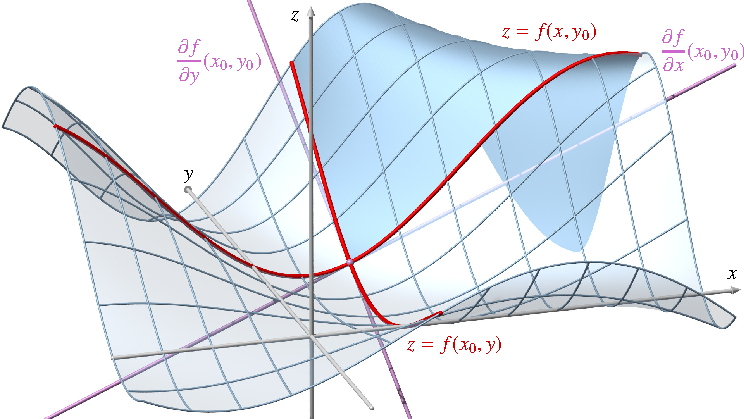
\includegraphics[width=\textwidth]{../slides/1/partabl.pdf}
\end{frame}
\egroup

Die partielle Funktion $x\mapsto f(x,y_0)$ hat als Graph die Schnittkurve
der Fläche mit der vertikalen Ebene $y=y_0$, entsprechend ist der Graph
der partiellen Funktion $y\mapsto f(x_0,y)$ die Schnittkurve der Fläche
mit der vertikalen Ebene $x=x_0$, beide Schnittkurven sind in
Abbildung~\ref{buch:fuvar:richtungsableitung:fig:partabl} rot hervorgehoben.

%
% Notation
%
\subsubsection{Notation}
Die in Definition~\ref{buch:fuvar:richtungsbleitung:def:partielleableitung}
eingeführte Notation ist intuitiv und erinnert an die Notation für den
Differentialquotienten einer Funktion einer Variablen.
Sie hat aber auch einen gravierenden Nachteil, der am Beispiel
der Funktion $f(x,y)$ illustriert werden soll.
Die partiellen Ableitungen der Funktion $f$ nach $x$ und $y$ sind
\[
\frac{\partial f}{\partial x}
\quad\text{und}\qquad
\frac{\partial f}{\partial y}.
\]
Setzt man die Argumentwerte $x^2+y^2$ und $x^2-y^2$ in die Funktion
$f$ ein, entsteht dann die Funktion
\begin{equation}
(x,y) \mapsto f(x^2+y^2,x^2-y^2).
\label{buch:fuvar:richtungsableitung:eqn:feingesetzt}
\end{equation}
Wie soll man die Ableitung dieser Funktion nach $x$ schreiben?
Und was soll die Notation
\[
\frac{\partial f}{\partial x}(x^2+y^2,x^2-y^2)
\]
bedeuten?
Ist dies die partielle Ableitung nach dem ersten Argument von $f$
oder ist es die Ableitung der zusammengesetzten Funktion nach $x$?

Offenbar wurden hier die Symbole $x$ und $y$ auf zwei verschiedene
Arten verwendet.
In der Schreibweise $f(x,y)$ ist das $x$ ein Platzhalter für die
erste Variable, das $y$ ist Platzhalter für die zweite Variable.
Die Symbole haben also vor allem syntaktische Eigenschaften.
Die Aussage, dass $f$ eine Funktion $\mathbb{R}^2\to\mathbb{R}$
ist, sagt genauso viel.
Die Variablen $x$ und $y$ werden nur gebraucht, wenn man zum
Beispiel mit einer Formel wie $f(x,y)=\sin x\cdot\cos y$ 
anzeigen will, wie ein Funktionswert berechnet werden soll.

In der Form~\eqref{buch:fuvar:richtungsableitung:eqn:feingesetzt} 
stehen aber $x$ und $y$ für beliebige reelle Zahlen.
Daraus müssen erst die Werte $x^2+y^2$ und $x^2-y^2$ berechnet werden,
die dann als erstes bzw.~zweites Argument der Funktion eingesetzt
werden müssen.
Die Notation~\eqref{buch:fuvar:richtungsableitung:eqn:feingesetzt} ist also
eigentlich eine abgekürzte Schreibweise für eine zusammengesetzte
Funktion, die sich aus
\[
g
\colon
\mathbb{R}^2 \to \mathbb{R}^2
:
(x,y) \mapsto (x^2+y^2,x^2-y^2)
\]
und der Funktion $f$ zusammensetzt.

\begin{beispiel}
\label{buch:fuvar:richtungsableitung:bsp:L}
In Abschnitt~\ref{buch:variation:section:eulerlagrange} werden wir
Extremalprobleme für Funktionen konstruieren, die als Integrale
einer Funktion $L$ von drei Variablen entstehen.
Zu jeder Funktion $y\colon \mathbb{R}\to\mathbb{R}:x\mapsto y(x)$
wird das Integral
\begin{equation*}
I
=
\int_a^b L(x,y(x),y'(x))\,dx
\end{equation*}
berechnet.
Die Funktion $L$ wird dabei meistens als $L(x,y,y')$ geschrieben.
Es wird dann die  Euler-Lagrange-Differentialgleichung abgeleitet,
in der die Ausdrücke
\begin{equation}
\frac{\partial L}{\partial y}
\qquad\text{und}\qquad
\frac{\partial L}{\partial y'}
\label{buch:fuvar:richtungsableitungen:eqn:Lderiv}
\end{equation}
auftreten.
Obwohl $y$ und $y'$ Funktionen von $x$ sind, sind mit den 
partiellen Ableitungen~\eqref{buch:fuvar:richtungsableitungen:eqn:Lderiv}
die Ableitungen nach der zweiten und dritten unabhängigen Variable
von $L$ gemeint.
\end{beispiel}

\begin{definition}
\label{buch:fuvar:richtungsableitung:def:D}
Sei $f\colon \mathbb{R}^n \to V$ eine Funktion von $n$ Variablen
mit Werten in einem endlichdimensionalen Vektorraum.
Die partielle Ableitung nach der $k$-ten Variable wird auch als
\[
D_kf(x_1,\dots,x_n)
=
\lim_{h\to 0}
\frac{f(x_1,\dots,x_k+h,\dots,x_n)-f(x_1,\dots,x_k,\dots,x_n)}{h}
\]
bezeichnet.
Manchmal wird auch die Notation $\partial_k f = D_kf$ verwendet.
\end{definition}

\begin{beispiel}
Mit der Notation von Definition~\ref{buch:fuvar:richtungsableitung:def:D}
werden die partiellen Ableitungen der Funktion $L(x,y,y')$ von
Beispiel~\ref{buch:fuvar:richtungsableitung:bsp:L} zu
\begin{align*}
\frac{\partial L}{\partial x}(x,y,y')
&=
D_1L(x,y,y'),
\\
\frac{\partial L}{\partial y}(x,y,y')
&=
D_2L(x,y,y')
\intertext{und}
\frac{\partial L}{\partial y'}(x,y,y')
&=
D_3L(x,y,y').
\end{align*}
Die neue Notation eliminiert die Zweideutigkeit.
$D_3L(x,y(x),y'(x))$ bedeutet, dass die Funktion $L$ zuerst partiell
nach der dritten Variable abgeleitet werden soll, dann sollen die
Werte $x$, $y(x)$ und $y'(x)$ als Argumente eingesetzt werden.
\end{beispiel}

%
% Lineare Ersatzfunktion
%
\subsubsection{Lineare Ersatzfunktion}
%
% tangentialebene.tex
%
% (c) 2024 Prof Dr Andreas Müller
%
\begin{figure}
\centering
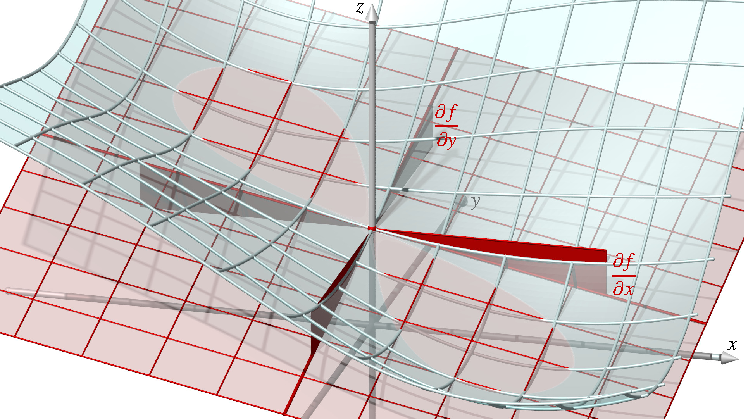
\includegraphics{chapters/010-fuvar/images/tangential.pdf}
%\includegraphics{chapters/010-fuvar/images/tangentialebene.pdf}
\caption{Mit den partiellen Ableitungen $\frac{\partial f}{\partial x}$
und $\frac{\partial f}{\partial y}$ einer Funktion lässt sich die rote
Tangentialebene in einem Punkt als lineare Ersatzfunktion konstruieren.
\label{buch:fuvar:richtungsableitung:fig:tangentialebene}}
\end{figure}

Die Ableitung einer Funktion wird manchmal auch als eine lineare
Ersatzfunktion definiert.

\begin{definition}
Eine Funktion $f\colon\mathbb{R}^n\to\mathbb{R}^m$ heisst {\em differenzierbar}
im Punkt $x_0\in\mathbb{R}^n$, wenn es eine lineare Funktion
$l\colon \mathbb{R}^n\to\mathbb{R}^m$ gibt mit der Eigenschaft, dass
\[
|f(x_0+\Delta x) - f(x_0) - l(\Delta x)| = o(\Delta x)
\]
ist.
Diese Notation bedeutet, dass
\[
\lim_{\Delta x\to 0}
\frac{o(\Delta x)}{\Delta x}
=
\lim_{\Delta x\to 0}
\frac{|f(x_0+\Delta x)-f(x_0)-l(\Delta x)|}{|\Delta x|}
=
0.
\]
Man sagt auch, eine $o(\Delta x)$-Funktion geht schneller gegen $0$ als
$\Delta x$.
\end{definition}

%
% Kettenregel
%
\subsubsection{Kettenregel}
Die Kettenregel ermöglicht, die Ableitungen zusammengesetzter Funktionen
zu berechnen.
Im vorliegenden Kontext der Funktionen mehrerer Variablen suchen
wir nach einer Regel, die Ableitungen einer zusammengesetzten Funktion
$f\circ g$
für zwei Funktionen
\[
g\colon \mathbb{R}^r\to\mathbb{R}^n
\qquad\text{und}\qquad
f\colon \mathbb{R}^n\to\mathbb{R}^m
\]
berechnet.
Die lineare Ersatzfunktion der Funktion $g$ ist jetzt durch
eine Matrix beschrieben.

\begin{definition}
\label{buch:fuvar:richtungsableitung:def:ableitungsmatrix}
Die partiellen Ableitungen einer Funktion
$g\colon\mathbb{R}^n\to\mathbb{R}^m$
kann als $m\times n$-Matrix
\[
Dg
=
\begin{pmatrix}
D_1g_1 & D_2g_1 & \dots  & D_ng_1 \\
D_1g_2 & D_2g_2 & \dots  & D_ng_2 \\
\vdots & \vdots & \ddots & \vdots \\
D_1g_m & D_2g_m & \dots  & D_ng_m
\end{pmatrix}
=
J_g
=
{\renewcommand{\arraystretch}{2.0}
\begin{pmatrix}
\displaystyle \frac{\partial g_1}{\partial x_1}
	&\displaystyle \frac{\partial g_1}{\partial x_2}
		&\dots
			&\displaystyle \frac{\partial g_1}{\partial x_n}
\\
\displaystyle \frac{\partial g_2}{\partial x_1}
	&\displaystyle  \frac{\partial g_2}{\partial x_2}
		&\dots
			&\displaystyle \frac{\partial g_2}{\partial x_n}
\\
\vdots	&\vdots	&\ddots	&\vdots \\
\displaystyle \frac{\partial g_m}{\partial x_1}
	&\displaystyle  \frac{\partial g_m}{\partial x_2}
		&\dots
			&\displaystyle \frac{\partial g_m}{\partial x_n}
\end{pmatrix}}
\]
gesschrieben werden.
Sie heisst auch die {\em Jacobi-Matrix}.
\index{Jacobi-Matrix}%
\end{definition}

Die Ableitung einer zusammengesetzten Funktion $f(g(x))$ einer 
Variable ist durch die Kettenregel
\[
(f\circ g)'(x)
=
f'(g(x)) g'(x)
\]
gegeben.
Für Funktionen mehrerer Variablen wird die Formel etwas komplizierter.

\begin{satz}
Seien $f\colon \mathbb{R}^m\to\mathbb{R}^n$ und
$g\colon\mathbb{R}^r\to\mathbb{R}^m$ Funktionen und sei zudem
$g$ im Punkt $x_0$ differenzierbar und $f$ im Punkt $g(x_0)$.
Dann ist die Zusammensetzung $f\circ g$ differenzierbar im Punkt $x_0$
und die Ableitungsmatrix ist
\[
D(f\circ g) = Df(g(x_0)) Dg(x_0).
\]
\end{satz}

Schreibt man $g(x)=y\in\mathbb{R}^m$ und ist $f(y)$ eine reellwertige Funktion,
dann hat $f$ die partiellen Ableitungen
\[
D_k(f\circ g)(x)
=
D_kf(g(x_0)) Dg(x_0)
=
\sum_{l=1}^m
\frac{\partial f}{\partial y_l}(g(x_0))
\frac{\partial y_l}{\partial x_k}(x_0).
\]
$Df$ ist eine $1\times m$-Matrix, $Dg$ ist eine $m\times r$-Matrix und
$D(f\circ g)$ ist einem $1\times r$-Matrix.

%
% Höhere Ableitungen
%
\subsubsection{Höhere Ableitungen}
Ist $f\colon U\to\mathbb{R}$ eine differenzierbare Funktion, dann ist
die Ableitung
\[
\partial_if\colon x\mapsto \frac{\partial f}{\partial x_i}(x)
\]
wieder eine stetige Funktion auf $U$, und man kann erneut die Frage
stellen, ob sie differenzierbar ist.
Die folgende rekursive Definition schafft einen handlichen Begriff
dafür.

\begin{definition}[Höhere partielle Ableitungen]
Eine Funktion $f\colon U\to\mathbb{R}$ mit $U\subset\mathbb{R}^n$ heisst
{\em $n$ mal differenzierbar}, wenn die partiellen Ableitungen
\[
\partial_i f
\colon
U\to\mathbb{R}
:
x\mapsto
\frac{\partial f}{\partial x_i}(x)
\]
für alle $i=1,\dots,n$ $n-1$-mal differenzierbar sind.
Sie heisst {\em $n$-mal stetig} differenzierbar, wenn alle partiellen
ersten Ableitungen $n-1$-mal stetig differenzierbar sind.
\end{definition}

Wenn eine Funktion zweimal differenzierbar ist, existieren alle
partiellen Ableitungen
\[
\frac{\partial^2 f}{\partial x_i\,\partial x_k},
\quad
i,k=1,\dots,n,
\]
es ist aber a priori alles andere als klar, ob die Reihenfolge der
Ableitungen eine Rolle spielt.
Der folgende Satz von Schwarz klärt diese Frage.

\begin{satz}[Schwarz]
Ist $f\colon U\to\mathbb{R}$ für eine offene Umgebung $U\subset\mathbb{R}^n$
eine zweimal stetig differenzierbare Funktion, dann kommt es bei
gemischten Ableitungen nicht auf die Reihenfolge an, es ist
\[
\frac{\partial^2 f}{\partial x_i\,\partial x_k}(x)
=
\frac{\partial^2 f}{\partial x_k\,\partial x_i}(x)
\]
für alle $x\in U$.
\end{satz}

Man beachte, dass der Satz nicht gilt, wenn die Ableitungen nur
existieren, aber nicht notwendigerweise stetig sind.
In diesem Fall lassen sich Gegenbeispiele konstruieren, wie
das folgende Beispiel von Schwarz zeigt.

\begin{beispiel}
\label{buch:fuvar:richtungsableitung:beispiel:schwarz}
%
% schwarz.tex -- Gegenbeispiel zum Satz von Schwarz
%
% (c) 2024 Prof Dr Andreas Müller
%
\begin{figure}
\centering
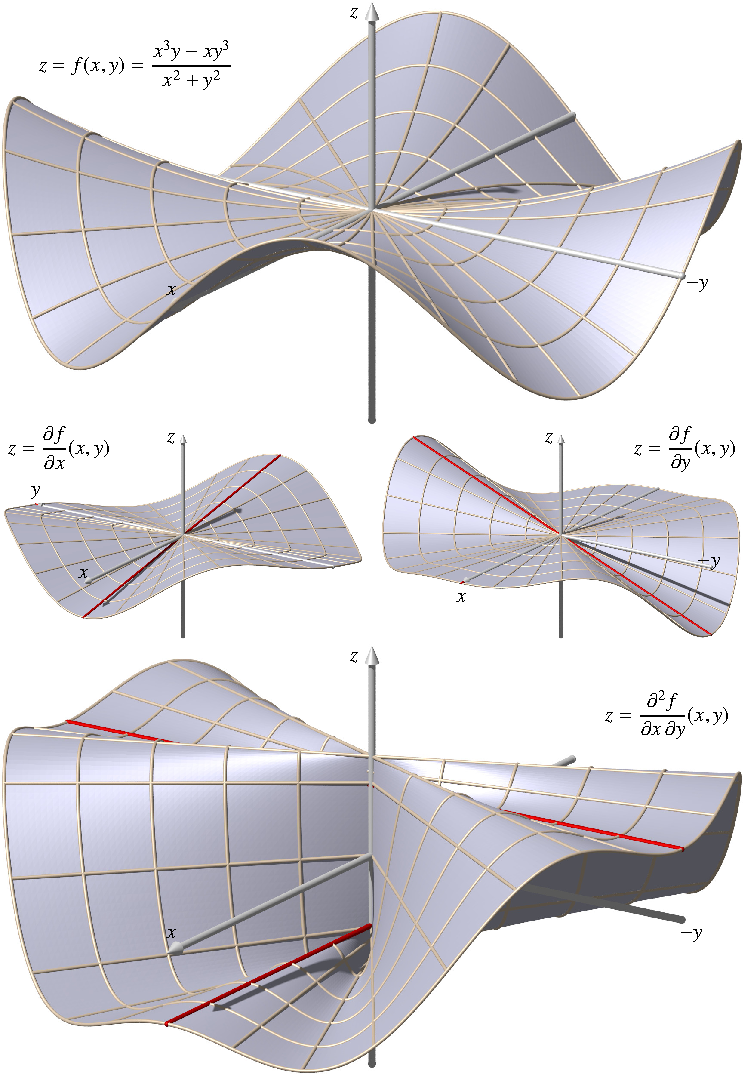
\includegraphics{chapters/010-fuvar/images/schwarz.pdf}
\caption{Gegenbeispiel~\ref{buch:fuvar:richtungsableitung:beispiel:schwarz}
zum Satz von Schwarz.
Oben der Graph der Funktion $f(x,y)$, in der Mitte die beiden 
ersten partiellen Ableitungen.
Die gemischten Ableitungen in der untersten Abbildung ist an der
Stelle $(x,y)=(0,0)$ nicht mehr stetig.
\label{buch:fuvar:richtungsableitung:fig:schwarz}}
\end{figure}

Wir betrachten die Funktion
\[
f
\colon
\mathbb{R}^2\to\mathbb{R}
:
(x,y)
\mapsto
f(x,y)
=
\begin{cases}
\displaystyle \frac{x^3y-xy^3}{x^2+y^2}&\qquad (x,y)\ne (0,0)\\
0&\qquad\text{sonst},
\end{cases}
\]
die auch in Abbildung~\ref{buch:fuvar:richtungsableitung:fig:schwarz}
zusammen mit den partiellen ersten Ableitungen und den gemischten
zweiten Ableitungen dargestellt ist.
Die Ableitungen im Nullpunkt sind
\begin{align*}
\frac{\partial f}{\partial x}(x,y)
&=
\frac{x^4y+4x^2y^3-y^5}{(x^2+y^2)^2}
&&\Rightarrow&
\frac{\partial f}{\partial x}(0,y)
&=
\frac{-y^5}{y^4} = -y
\\
\frac{\partial f}{\partial y}(x,y)
&=
\frac{x^5-4x^3y^2-xy^4}{(x^2+y^2)^2}
&&\Rightarrow&
\frac{\partial f}{\partial y}(x,0)
&=
\frac{x^5}{x^4}
=
x.
\intertext{Sie sind in Abbildung~\ref{buch:fuvar:richtungsableitung:fig:schwarz}
in der Mitte rot hervorgehoben.
Daraus ergeben sich die zweiten Ableitungen}
\frac{\partial^2 f}{\partial y\,\partial x}(0,y)
&=
\frac{\partial}{\partial y}(-y)
=
-1
&&\Rightarrow&
\frac{\partial^2 f}{\partial y\,\partial x}(0,0)
&=
-1
\\
\frac{\partial^2 f}{\partial x\,\partial y}(x,0)
&=
\frac{\partial}{\partial x}(x)
=
1
&&\Rightarrow&
\frac{\partial^2 f}{\partial x\,\partial y}(0,0)
&=
1.
\end{align*}
Die erste Gleichung entspricht den roten Geraden über der $y$-Achse
in Abbildung~\ref{buch:fuvar:richtungsableitung:fig:schwarz},
die zweite entspricht den roten Geraden über der $x$-Achse.
Die roten Geraden zeigen daher gemischte zweite Ableitungen in
verschiedenen Differentiationsreihenfolgen mit verschiedenen
Werten.
Somit sind die Grenzwerte an der Stelle $(0,0)$ verschieden und
die Funktion der gemischten Ableitungen ist nicht stetig an der Stelle
$(0,0)$.

Die Abbildung~\ref{buch:fuvar:richtungsableitung:fig:schwarz}
zeigt auch, dass die Funktionsgraphen von $\frac{\partial f}{\partial x}$
und $\frac{\partial f}{\partial y}$ im Nullpunkt keine lineare
Ersatzfunktion haben.
\end{beispiel}

%
% Richtungsableitung
%
\subsection{Richtungsableitung}
Die partiellen Ableitungen einer Funktion $f(x_1,\dots,x_n)$
nach der Variablen $x_k$ entstehen dadurch, dass alle Variablen
ausser $x_k$ konstant gehalten werden und die so entstehende
Funktion der einzigen Variablen $x_k$ abgeleitet wird.
%
% richtungsableitung.tex -- Richtungsableitung einer Funktion f(x,y)
%
% (c) 2024 Prof Dr Andreas Müller
%
\begin{figure}
\centering
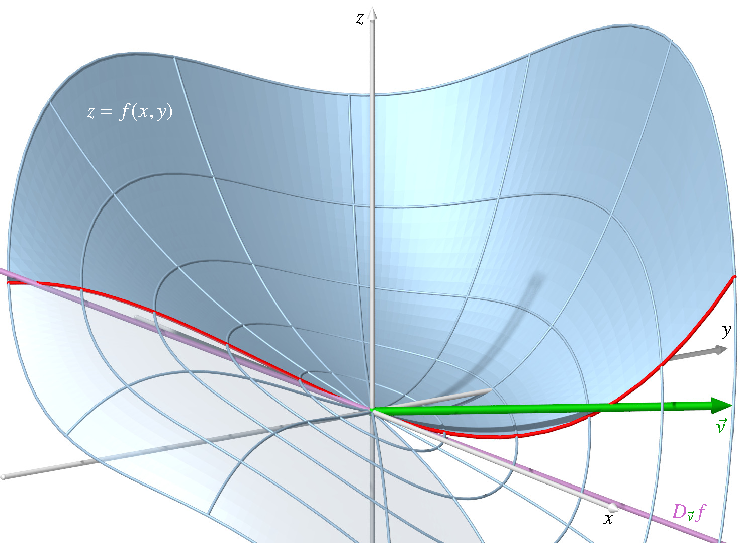
\includegraphics{chapters/010-fuvar/images/richtungsabl.pdf}
\caption{Definition der Richtungsableitung einer Funktion $f(x,y)$
zweier Variablen in Richtung des {\color{darkgreen}grünen}
Vektors ${\color{darkgreen}\vec{v}}$.
Die Richtungsableitung ist die Steigung der {\color{darkred}roten}
Schnittkurve der vertikalen Ebene mit Richtung ${\color{darkgreen}\vec{v}}$ 
und der Fläche des Graphen $z=f(x,y)$.
\label{buch:fuvar:richtungsableitung:fig:richtungsableitung}}
\end{figure}

%
% partrichtung.tex
%
% (c) 2024 Prof Dr Andreas Müller
%
\begin{figure}
\centering
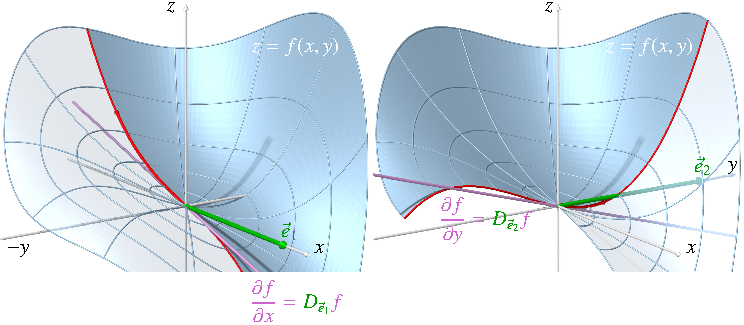
\includegraphics{chapters/010-fuvar/images/fxy.pdf}
\caption{Die partiellen Ableitungen sind Richtungsableitungen der
Funktion in Richtung der Koordinatenachsen.
\label{buch:fuvar:richtungsableitung:fig:partrichtung}}
\end{figure}

Die Funktion $f$ kann aber noch auf eine andere Art zu einer
Funktion nur einer Variablen gemacht werden.
Dazu verwendet man die Parameterdarstellung $x(t) = x + vt$ einer
Geraden durch den Punkt $x$ mit Richtungsvektor $v$
(Abbildung~\ref{buch:fuvar:richtungsableitung:fig:richtungsableitung}).
Die Funktion $f(x+vt)$ hängt nur noch von der Variablen $t$ ab
und kann wie gewohnt nach $t$ abgeleitet.

\begin{definition}
\label{buch:fuvar:richtungsableitung:def:richtungsableitung}
Die {\em Richtungsableitung} der Funktion $f\colon\mathbb{R}^n\to\mathbb{R}^m$
\index{Richtungsableitung}%
im Punkt $x\in\mathbb{R}^n$ in Richtung $v\in\mathbb{R}^n$ ist 
\[
D_vf(x)
=
\frac{d}{dt}f(x+tv)\bigg|_{t=0}.
\]
\end{definition}

Die Notation für die Richtungsableitung von
Definition~\ref{buch:fuvar:richtungsableitung:def:richtungsableitung}
konkurriert mit der Notation für die partiellen Ableitungen von
Definition~\ref{buch:fuvar:richtungsableitung:def:D}.
Tatsächlich entsteht aber kein Widerspruch, denn die 
Richtungsableitung in Richtung des Standardbasisvektors $e_k$ ist
\begin{align*}
D_{e_k}f(x)
&=
\frac{d}{dt} f(x+te_k)\bigg|_{t=0}
\\
&=
\lim_{h\to 0}
\frac{f(x_1,\dots,x_k+t,\dots,x_n)-f(x_1,\dots,x_k,\dots,x_n)}{h}
\\
&=
D_kf(x)
\end{align*}
oder kurz $D_{e_k}=D_k$
(siehe auch Abbildung~\ref{buch:fuvar:richtungsableitung:fig:partrichtung}).

Die Ableitung der Funktion $t\mapsto x+vt$ für $x\in\mathbb{R}^n$
und $v\in\mathbb{R}^n$ nach der einen Variablen $t$ ist
\[
\frac{d}{dt}
\begin{pmatrix}
x_1+v_1t\\
x_2+v_2t\\
\vdots  \\
x_n+v_nt
\end{pmatrix}
=
\begin{pmatrix}
v_1\\
v_2\\
\vdots\\
v_n
\end{pmatrix}.
\]
Damit kann die Richtungsableitung einer Funktion
$f\colon\mathbb{R}^n\to\mathbb{R}$
im Punkt $x\in\mathbb{R}^n$ mit der Kettenregel als
\begin{equation}
D_vf(x)
=
\frac{\partial f}{\partial x_1}(x)\, v_1
+
\dots
+
\frac{\partial f}{\partial x_n}(x)\, v_n
=
\sum_{k=1}^n \frac{\partial f}{\partial x_k}\, v_k
\label{buch:fuvar:richtungsableitung:eqn:richtungsableitungkette}
\end{equation}
berechnet werden.

%
% Gradient
%
\subsection{Gradient}
Die Schreibweise
\eqref{buch:fuvar:richtungsableitung:eqn:richtungsableitungkette}
für die Richtungsableitung der Funktion $f\colon\mathbb{R}^n\to\mathbb{R}$
lässt sich auch als Skalarprodukt des Vektors $v$ mit einem Vektor
bestehend aus den partiellen Ableitungen schreiben.

\begin{definition}
\label{buch:fuvar:richtungsableitung:def:gradient}
Der {\em Gradient} der Funktion $f\colon\mathbb{R}^n\to\mathbb{R}$ ist der
Vektor
\[
\operatorname{grad}f(x)
=
{
\renewcommand{\arraystretch}{1.9}
\begin{pmatrix}
\displaystyle
\frac{\partial f}{\partial x_1}(x)\\
\displaystyle
\frac{\partial f}{\partial x_2}(x)\\
\vdots \\
\displaystyle
\frac{\partial f}{\partial x_n}(x)
\end{pmatrix}
}
\]
\index{Gradient}
\end{definition}

Der Gradient ist auch die transponierte Matrix der Jacobi-Matrix:
$\operatorname{grad}f(x) = \transpose{Df(x)} = \transpose{J_f(x)}$.
Als weitere Notation ist ausserdem der Nabla-Operator gemäss der folgenden
Definition verbreitet.

\begin{definition}[Nabla-Operator]
\label{buch:fuvar:richtungsableitung:def:nabla}
Der {\em Nabla-Operator} ist der Differentialoperator
\index{Nabla-Operator}%
\index{Operator!Nabla-}%
\[
\nabla 
=
{
\renewcommand{\arraystretch}{1.8}
\begin{pmatrix}
\displaystyle
\frac{\partial}{\partial x_1}\\
\displaystyle
\frac{\partial}{\partial x_2}\\
\vdots\\
\displaystyle
\frac{\partial}{\partial x_n}
\end{pmatrix}
}
\]
auf Funktionen
$\mathbb{R}^n\to\mathbb{R}$, der durch
\[
\nabla f
=
{
\renewcommand{\arraystretch}{1.9}
\begin{pmatrix}
\displaystyle
\frac{\partial f}{\partial x_1}(x)\\
\displaystyle
\frac{\partial f}{\partial x_2}(x)\\
\vdots\\
\displaystyle
\frac{\partial f}{\partial x_n}(x)
\end{pmatrix}
}
=
\operatorname{grad}f(x)
\]
definiert ist.
\end{definition}




%
% 2-kritisch.tex
%
% (c) 2023 Prof Dr Andreas Müller
%
\section{Kritische Punkte
\label{buch:fuvar:section:kritisch}}
\kopfrechts{Kritische Punkte}

\begin{verbatim}
- verschwindende erste Ableitungen
- notwendige Bedingung für Extremum
- Orthogonalität
\end{verbatim}

%
% 3-nebenbedingungen.tex
%
% (c) 2023 Prof Dr Andreas Müller
%
\section{Nebenbedingungen
\label{buch:fuvar:section:kritisch}}
\kopfrechts{Nebenbedingungen}
Die Nullstellen des Gradienten sind Kandidaten für die Lösung
des Extremalproblems einer Funktion $f\colon\mathbb{R}^n\to\mathbb{R}$.
Oft trifft man jedoch Situation, in denen sich das Argument
$x\in\mathbb{R}^n$ der Funktion $f(x)$ nur auf einer Teilmenge
bewegen darf.
In diesem Abschnitt soll ein Verfahren beschrieben werden, wie sich
ein solches Problem exakt formulieren und lösen lässt.

%
% Nebenbedingungen
%
\subsection{Nebenbedingungen}
Wir betrachten das folgende Problem als Beispiel, wie sich 
Nebenbedingungen formulieren lassen.

%
% Ein Extremalproblem auf einer Kugeloberfläche
%
\subsubsection{Ein Extremalproblem auf einer Kugeloberfläche}
Auf der Oberfläche der Einheitskugel mit Mittelpunkt im Nullpunkt
des $(x_1,x_2,x_3)$-Koor\-di\-na\-ten\-sys\-tems sind die Extrema
der Funktion 
\begin{equation}
f(x)
=
x_2^2
-
x_1x_2
-
x_1x_3
-
x_2x_3
\label{buch:fuvar:nebenbedingungen:eqn:beispielf}
\end{equation}
zu finden.

%
% Lösung durch Umparametrisierung
%
\subsubsection{Lösung durch Umparametrisierung}
Eine erster Lösungsansatz ist, die Kugeloberfläche mit Kugelkoordinaten
\[
\begin{pmatrix}
x_1\\
x_2\\
x_3
\end{pmatrix}
=
\begin{pmatrix}
\sin\vartheta\cos\varphi\\
\sin\vartheta\sin\varphi\\
\cos\vartheta
\end{pmatrix}
\]
zu parametrisieren.
Durch Einsetzen der Parametrisierung in
\eqref{buch:fuvar:nebenbedingungen:eqn:beispielf}
entsteht die Funktion
\begin{align*}
f(\varphi,\vartheta)
&=
\sin^2\vartheta
\sin\varphi
(\sin\varphi
-
\cos\varphi)
-
(
\cos\varphi
+
\sin\varphi
)
\sin\vartheta
\cos\vartheta.
\end{align*}
Das Problem ist damit zu einem Extremalproblem in zwei Dimensionen
geworden und kann mit den bereits behandelten Methoden gelöst werden.

%
% Zusätzliche Bedingungen
%
\subsubsection{Zusätzliche Bedingungen}
Der Lösungsansatz durch Umparametrisierung wird weiter erschwert,
wenn zusätzliche Bedingungen erfüllt werden muss.
Wird zusätzlich Verlangt, dass der Punkt $x\in\mathbb{R}^3$ auf
dem Ellipsoid mit der Gleichung
\begin{equation}
g(x)
=
\begin{pmatrix}
x_1\\x_2\\x_3
\end{pmatrix}^t
\begin{pmatrix}
2&1&1\\
1&3&1\\
1&1&4
\end{pmatrix}
\begin{pmatrix}
x_1\\x_2\\x_3
\end{pmatrix}
=
1.
\label{buch:fuvar:nebenbedingungen:eqn:beispielg},
\end{equation}
liegt, dann werden die zulässigen Punkte durch eine Kurve in der
$(\varphi,\vartheta)$-Ebene beschrieben, für die eine Parametrisierung
gefunden werden muss.
Eine solche Lösung ist offenbar sehr kompliziert.
Gesucht wird ein Lösungsansatz, der ohne Umparametrisierung das folgende
allgemeine Problem löst.

\begin{aufgabe}
\label{buch:fuvar:nebenbedingungen:aufgabe:grund}
Gegeben sind stetig differenzierbare Funktionen
$f\colon\mathbb{R}^n\to\mathbb{R}$ und
$g_i\colon\mathbb{R}^n\to\mathbb{R}$ für $i=1,\dots,k$.
Man finde ein Extremum der Funktion $f(x)$ unter der Bedingungen,
dass
\[
g_1(x) = 0,\quad g_2(x)=0,\quad\dots,\quad g_k(x)=0
\]
gilt.
\end{aufgabe}

%
% Extremalaufgaben mit einer Nebenbedingung
%
\subsection{Extremalaufgaben mit einer Nebenbedingung}
In diesem Abschnitt untersuchen wir das Extremum einer stetig
differenzierbaren Funktion $f\colon\mathbb{R}^n\to\mathbb{R}$
unter der Bedinung $g(x)=0$ mit einer stetig differenzierbaren
Funktion $g\colon\mathbb{R}^n\to\mathbb{R}$.
Sei also $x_0\in\mathbb{R}^n$ so, dass $f(x_0)$ minimal ist unter
allen Punkten $x\in \mathbb{R}^n$, die die Nebenbedingungen $g(x)=0$
erfüllen.
Da $x_0$ ein Minimum ist, müssen die Werte $f(x)$ für Punkte $x$
in der Nähe von $x_0$ grösser sein, allerdings nur, wenn $x$ auch
die Bedingungen $g(x)=0$ erfüllt.

Für ein Extremalproblem ohne Nebenbedingung wurde das Verschwinden
aller Richtungsableitung als notwendige Bedingung für das
Extremum gefunden.
Tatsächlich nimmt die Funktion auch in jeder Richtung ausgehend
von $x_0$ zu.
Unter der Nebenbedingung gilt dies nicht mehr.
Nur noch Änderungen von $x$, die auch die Nebenbedingung
erfüllen, durfen in Betracht gezogen werden.
Die von $x_0$ ausgehdenden Geraden $t\mapsto x_0+vt$ mit dem
Richtungsvektor $v$ erfüllen die Nebenbedingungen nur dann, wenn
die Menge $M=\{x\in\mathbb{R}^n \mid g(x)=0\}$ Geraden enthält, also
typischerweise gar nicht.

Es müssen also Kurven $t\mapsto x(t)\in\mathbb{R}^n$ mit $x(0)=x_0$
betrachtet werden, die $g(x(t))=0$ für alle $t$ in einer kleinen Umgebung
von $0$ erfüllen.
Für ein Minimum ist dann notwendig, dass die Ableitung
\begin{equation}
0
=
\frac{d}{dt} f(x(t))\bigg|_{t=0}
=
Df(x_0)\cdot \frac{dx(t)}{dt}\bigg|_{t=0}
=
Df(x_0)\cdot \dot{x}(0)
\label{buch:fuvar:nebenbedingungen:eqn:gradf}
\end{equation}
ist.
Nicht jeder Vektor $v=\dot{x}$ kann vorkommen, da $\dot{x}(0)$ ein
Tangentialvektor der Menge $M$ ist.
Da $g(x(t))=0$ ist, sind diese Vektoren durch
\begin{equation}
0
=
\frac{d}{dt}g(x(t))\bigg|_{t=0}
=
Dg(x_0)\cdot \dot{x}(0)
=
\grad g(x_0)\cdot \dot{x}(0)
\label{buch:fuvar:nebenbedingungen:eqn:gradg}
\end{equation}
charakterisiert.
Nur Vektoren $\dot{x}(0)$, die auf dem Gradienten $\grad g(x_0)$ 
senkrecht stehen, sind zulässig.
Wir halten dieses Resultat im folgenden Lemma fest.

\begin{lemma}
\label{buch:fuvar:nebenbedingungen:lemma:nebenbedingungen}
Ist $x_0$ ein Extremum der Funktion $f(x)$ unter der Nebenbedingung
$g(x)=0$, dann verschwindet die Richtungsableitung
\(
D_vf(x_0) = \grad f(x_0)\cdot v = 0
\)
von $f$ an der Stelle $x_0$ in jeder Richtung $v$, die tangential
an die Menge $\{x\in\mathbb{R}^n \mid g(x)=0\}$ ist, für die also
$\grad g(x_0)\cdot v=0$ gilt.
\end{lemma}

Damit haben wir die folgende notwendige Bedingung gefunden.

\begin{satz}
Sei $f\colon\mathbb{R}^n\to\mathbb{R}$ eine stetig differenzierbare
Funktion, die im Punkt $x_0\in\mathbb{R}^n$ unter allen Punkten
$x\in\mathbb{R}^n$ ein Extremum annimmt unter der Nebenbedingung
$g(x)=0$ für eine stetig differenzierbare Funktion
$g\colon\mathbb{R}^n\to\mathbb{R}$ mit nicht verschwindendem Gradienten.
Dann ist $\grad{f}(x_0)$ ein Vielfaches von $\grad{g}(x_0)$.
\end{satz}

\begin{proof}
Nach
\eqref{buch:fuvar:nebenbedingungen:eqn:gradf}
und
\eqref{buch:fuvar:nebenbedingungen:eqn:gradg}
muss 
\[
\grad f(x_0)\cdot v = 0
\]
sein für alle Vektoren $v$ mit $\grad g(x_0)\cdot v= 0$.
Der Vektor $\grad f(x_0)$ steht also auf allen Vektoren senkrecht, die
auf $\grad g(x_0)$ senkrecht stehen.
Dies trifft wegen $\grad g(x_0)\ne 0$ genau dann zu, wenn $\grad f(x_0)$
ein Vielfaches von $\grad g(x_0)$ ist.
\end{proof}

\begin{beispiel}
Wir lösen die eingangs gestellte Aufgabe, die Extrema der Funktion
$f(x)$ von \eqref{buch:fuvar:nebenbedingungen:eqn:beispielf}
unter der Nebenbedingung zu finden, dass $|x|=1$ ist.
Die Funktion $g(x)$ ist
\[
g(x)
=
x_1^2 + x_2^2 + x_3^2 - 1.
\]
Die Gradienten von $f$ und $g$ sind
\[
\grad f(x)
=
\begin{pmatrix*}[r]
-x_2-x_3\\
-x_1+2x_2-x_3\\
-x_1-\phantom{2}x_2\phantom{\mathstrut-x_3}
\end{pmatrix*}
\qquad\text{und}\qquad
\grad g(x)
=
\begin{pmatrix}
2x_1\\
2x_2\\
2x_3
\end{pmatrix}
=
2x.
\]
Kandidaten für Extremale sind Punkte, in denen die beiden Gradienten
proportional sind, für die also das Gleichungssystem
\begin{equation}
\left.
\begin{aligned}
\grad f({\color{darkred}x})&=\lambda \grad g({\color{darkred}x})\\
      g({\color{darkred}x})&=0
\end{aligned}
\right\}
\quad\Rightarrow\quad
\left\{
\renewcommand\arraycolsep{2pt}
\begin{array}{rcrcrcr}
	&-& {\color{darkred}x_2}
		&-& {\color{darkred}x_3}
			&=& 2{\color{darkred}\lambda x_1}\\
-{\color{darkred}x_1}
	&+& 2{\color{darkred}x_2}
		&-& {\color{darkred}x_3}
			&=& 2{\color{darkred}\lambda x_2}\\
-{\color{darkred}x_1}
	&-& {\color{darkred}x_2}
		& &
			&=& 2{\color{darkred}\lambda x_3}\\
{\color{darkred}x}^2_{\color{darkred}1}
	&+& {\color{darkred}x}^2_{\color{darkred}2}
		&+& {\color{darkred}x}^2_{\color{darkred}3}
			&=& 1
\end{array}
\right.
\label{buch:fuvar:nebenbedingungen:eqn:glsystem}
\end{equation}
Dies ist ein System von vier nichtlinearen Gleichungen für die vier
Unbekannten ${\color{darkred}x_1}$, ${\color{darkred}x_2}$,
${\color{darkred}x_3}$ und ${\color{darkred}\lambda}$.
In Matrixform lassen sich die ersten drei Gleichungen als
\begin{equation}
\underbrace{
\begin{pmatrix*}[r]
 0&-1&-1\\
-1& 2&-1\\
-1&-1& 0
\end{pmatrix*}
}_{\displaystyle = A}
{\color{darkred}x}
=
A
{\color{darkred}x}
=
2{\color{darkred}\lambda x}
\label{buch:fuvar:nebenbedingungen:eqn:evgl}
\end{equation}
schreiben.
Da die vierte Gleichung von~\eqref{buch:fuvar:nebenbedingungen:eqn:glsystem}
verlangt, dass $\color{darkred}x$ nicht der Nullvektor ist, besagt
\eqref{buch:fuvar:nebenbedingungen:eqn:evgl}, dass ${\color{darkred}}$
ein Eigenvektor von $A$ mit Eigenwert $2{\color{darkred}\lambda}$ sein muss.
Das charakteristische Polynom
\[
\det(A-tI)
=
-t^3+2t^2+3t-4
=
-(t-1)(t^2+t-4)
\]
hat die Nullstellen $t_0=1$ und
\[
t_{\pm}
=
\frac{-1\pm\sqrt{17}}{2},
\]
was auf die zulässigen Werte
\[
{\color{darkred}\lambda}_0=-\frac12,
\quad\text{und}\quad
{\color{darkred}\lambda}_\pm = \frac{1\mp\sqrt{17}}{4}
\]
für ${\color{darkred}\lambda}$ führt.
Mit etwas Geduld oder einem Computeralgebrasystem kann man auch die
zugehörigen Eigenvektoren
\[
{\color{darkred}x}_0
=
\begin{pmatrix*}[r]
 1\\
 0\\
-1
\end{pmatrix*}
\quad\text{und}\quad
{\color{darkred}x}_\pm
=
\begin{pmatrix*}
1\\
\frac{-3\pm\sqrt{17}}{2}\\
1
\end{pmatrix*}
\]
finden.
Durch Normierung lassen sich jetzt Punkte finden, die die Nebenbedingung
erfüllen und damit Kandidaten für Extrema sind.
\end{beispiel}

%
% Lagrange-Multiplikatoren
%
\subsection{Lagrange-Multiplikatoren}
Wir kehren zum allgemeinen Problem der
Aufgaben~\ref{buch:fuvar:nebenbedingungen:aufgabe:grund}
zurück.
Sei also wieder $f\colon \mathbb{R}^n\to\mathbb{R}$
und
$g_i\colon\mathbb{R}^n\to\mathbb{R}$, $i=1,\dots,k$,
stetig differenzierbare Funktionen und $x_0$ ein Extremum
von $f$ unter allen $x\in\mathbb{R}^n$ mit $g_i(x)=0$ für $i=1,\dots,k$.
Die Richtungsableitung von $f$ an der Stelle $x_0$ muss für alle
Richtungen $v$ verschwinden, die tangential an die Menge
\[
M
=
\{
x\in\mathbb{R}^n
\mid
g_1(x)=\ldots=g_k(x)=0
\}
\]
sind.
Die zulässigen Richtungen $v$ erfüllen die Bedingung
\[
\grad g_i(x_0)\cdot v  = 0,\quad i=1,\dots,k,
\]
In Matrixform sind dies die Lösungen des homogenen Gleichungssystems
\[
{\renewcommand{\arraystretch}{1.2}
\begin{pmatrix}
\displaystyle\frac{\partial g_1}{\partial x_1}(x_0)
&\dots&
\displaystyle\frac{\partial g_1}{\partial x_n}(x_0)
\\
\vdots&\ddots&\vdots\\
\displaystyle\frac{\partial g_k}{\partial x_1}(x_0)
&\dots&
\displaystyle\frac{\partial g_k}{\partial x_n}(x_0)
\end{pmatrix}}
\begin{pmatrix}
v_1\\
\vdots\\
v_n
\end{pmatrix}
=
Dg(x_0) v
=
0.
\]

\begin{satz}
\label{buch:fuvar:nebenbedingungen:satz:lm}
Seien $f\colon\mathbb{R}^n\to\mathbb{R}$ und
$g_i\colon\mathbb{R}^n\to\mathbb{R}$, $i=1,\dots,k$, stetig
differenzierbare Funktionen.
Für ein Extremum $x_0$ von $f(x)$ unter allen $x\in\mathbb{R}^n$,
die die Nebenbedingungen $g_i(x)=0$, $i=1,\dots,k$ erfüllen, ist notwendig,
dass es reelle Zahlen $\lambda_1,\dots,\lambda_k\in\mathbb{R}$ gibt derart,
dass
\[
\grad f(x_0)
=
\lambda_1\grad g_1(x_0)
+\ldots+
\lambda_k\grad g_k(x_0)
=
\sum_{i=1}^k \lambda_i \grad g_i(x_0)
\]
gilt.
Kandidaten für Extrema von $f$ unter den Nebenbedingungen $g_i(x)=0$ sind
daher Lösungen des Gleichungssystems
\begin{equation}
\begin{aligned}
\grad f({\color{darkred}x})
&=
\sum_{i=1}^k {\color{darkred}\lambda_i} g_i({\color{darkred}x})
\\
g_i({\color{darkred}x})
&= 
0\qquad i=1,\dots k
\end{aligned}
\label{buch:fuvar:nebenbedingungen:eqn:lm}
\end{equation}
für ${\color{darkred}x}$ und ${\color{darkred}\lambda_i}$, $i=1,\dots,k$.
\end{satz}

Die erste Gleichung des Gleichungssytems
\eqref{buch:fuvar:nebenbedingungen:eqn:lm}
ist eine $n$-dimensionale Vektorgleichung, entspricht also $n$
Komponentengleichungen.
Sie kann auch geschrieben werden als ein lineares Gleichungssystem
mit $n$ Gleichungen für die Variablen
${\color{darkred}\lambda_1},\dots,{\color{darkred}\lambda_k}$
mit der Koeffizientenmatrix $Dg(x_0)^t$.
Die Nebenbedingungen steuern $k$ weitere Gleichungen bei.
Insgesamt ist \eqref{buch:fuvar:nebenbedingungen:eqn:lm}
daher ein im Allgemeinen nichtlineares Gleichungssystem von $n+k$
Gleichungen für die $n+k$ Unbekannten
\(
{\color{darkred}x_1},\dots,{\color{darkred}x_n},
{\color{darkred}\lambda_1},\dots,{\color{darkred}\lambda_k}
\).
Leider kann man keine allgemeinen Lösungsverfahren für solche
Gleichungen erwarten.
Eine interessante Ausnahme liegt vor, wenn die Funktionen $f$ und $g_i$
quadratische Funktionen sind, dies wird im
Abschnitt~\ref{buch:fuvar:section:quadratisch}
untersucht.

Alternativ kann man den Satz
\ref{buch:fuvar:nebenbedingungen:satz:lm}
auch so formulieren:

\begin{satz}
\label{buch:fuvar:nebenbedingungen:satz:lm2}
Unter den Voraussetzungen von Satz~\eqref{buch:fuvar:nebenbedingungen:satz:lm}
ist für ein Extremum von $f$ unter den Nebenbedingungen $g_i$, $i=1,\dots,k$,
notwendig, dass es
es relle Zahlen $\lambda_1,\dots,\lambda_k\in\mathbb{R}$ derart gibt,
dass 
\[
\grad\biggl(f-\sum_{i=1}^k \lambda_ig_i\biggr)(x_0) = 0
\qquad\text{und}\qquad
g_i(x_0)=0\quad \forall i=1,\dots,k
\]
gilt.
\end{satz}


%
% 4-hessesche.tex
%
% (c) 2023 Prof Dr Andreas Müller
%
\section{Hessesche Matrix
\label{buch:fuvar:section:hessesche}}
\kopfrechts{Hessesche Matrix}
Das Verschwinden der Ableitung einer differenzierbaren Funktion
$f\colon\mathbb{R}\to\mathbb{R}$ ist eine notwendige Bedingung
für ein Extremum, sie ist aber nicht hinreichend.
Im Grundlagenunterricht in der Analysis lernt man, dass man mit
Hilfe der zweiten Ableitung zu einem hinreichenden Kriterium
kommen kann.
Ist die zweite Ableitung $f''(x_0)$ an einer Stelle $x_0$ grösser
als $0$, dann liegt ein Minimum vor, falls sie negativ ist, liegt
ein Maximum vor.
In diesem Abschnitt soll gezeigt werden, wie dieses Kriterium auf
Funktionen mehrere Variablen verallemeinert werden kann.

%
% Die zweite Ableitung
%
\subsection{Die zweite Ableitung}
In diesem Abschnitt ist $f\colon\mathbb{R}^n\to\mathbb{R}$
eine zweimal stetig differenzierbare Funktionen, deren Gradient
an der Stelle $x_0$ verschwindet.
Durch eine Translation $x\mapsto x-x_0$ kann man immer erreichen,
dass $x_0=0$ der Nullpunkt des Koordinatensystems ist.
In der folgenden Diskussion wird diese Konvention wo zweckmässig
stillschweigend verwendet.

%
% Die Hessesche Matrix
%
\subsubsection{Die Hessesche Matrix}
Damit der Punkt $x_0$ ein Minimum ist, muss jede auf die Richtung
$v\in\mathbb{R}^n$ eingeschränkte Funktion eine positive zweite
Ableitung haben.
Es muss also für alle $v\in\mathbb{R}^n$
\[
\frac{d^2}{dt^2} f(x_0+vt)\bigg|_{t=0}
> 0
\]
sein.
Wenn das umgekehrte Zeichen gilt, dann liegt ein Maximum vor.
Ausgeschrieben in Komponenten gilt
\[
\frac{d^2}{dt^2} f(x_0+vt)
=
\sum_{i,k=1}^n
\frac{\partial^2 f}{\partial x_i\,\partial x_k}(x_0+vt)
\,
v_iv_k,
\]
wobei die $v_i$ die Komponenten von $v$ sind.
An der Stelle $t=0$ bleibt die Eigenschaft
\[
\frac{d^2}{dt^2}f(x_0+vt)\bigg|_{t=0}
=
\sum_{i,k=1}^n \frac{\partial^2 f}{\partial x_i\,\partial x_k}(x_0) \,v_iv_k
>
0.
\]
Die Summe kann mit Hilfe der Matrix $H$ mit den Einträgen
\[
h_{ik}
=
\frac{\partial^2 f}{\partial x_i\,\partial x_k}(x_0)
\]
kompakter als
\[
\frac{d^2}{dt^2}f(x_0+vt)\bigg|_{t=0}
=
\sum_{i,k=1}^n \frac{\partial^2 f}{\partial x_i\,\partial x_k}(x_0) \,v_iv_k
=
v^tHv
>
0
\]
geschrieben werden.
Ein hinreichendes Kriterium für ein Minimum wird also zu einer
Eigenschaft der Matrix $H$.

\begin{definition}[Hessesche Matrix]
Ist $f\colon\mathbb{R}^n\to\mathbb{R}$ eine zweimal stetig differenzierbare
Funktion, dann heisst die Matrix
\[
H(x_0)
=
\begin{pmatrix}
h_{11}(x_0)&\dots &h_{1n}(x_0)\\
\vdots&\ddots&\vdots\\
h_{n1}(x_0)&\dots &v_{nn}(x_0)
\end{pmatrix}
\qquad\text{mit}\qquad
h_{ik}(x_0)
=
\frac{\partial^2 f}{\partial x_i\,\partial x_k}(x_0)
\]
die {\em hessesche Matrix}.
\index{hessesche Matrix}%
\end{definition}

Da die Funktion $f$ zweimal stetig differenzierbar angenommen wurde,
sind die partiellen Ableitungen nach dem Satz von Schwarz
\[
\frac{\partial^2 f}{\partial x_i\,\partial x_k}(x_0)
=
\frac{\partial^2 f}{\partial x_k\,\partial x_i}(x_0)
\]
vertauschbar.
Die hessesche Matrix $H(x_0)$ ist daher immer symmetrisch: $H(x_0)^t=H(x_0)$.

%
% Hinreichendes Kriterium für ein Extremum
%
\subsubsection{Hinreichendes Kriterium für ein Extremum}
Das Vorzeichen von $v^tH(x_0)v$ entscheidet darüber, ob ein Extremum
vorliegt.
Dies führt auf die folgende Definition.

\begin{definition}
Eine symmetrische Matrix $A$ heisst {\em positiv definit}, wenn 
\index{positiv definit}%
\index{definit, positiv}%
$v^tAv>0$ für alle Vektoren $v\in\mathbb{R}^n\setminus\{0\}$ ist.
Sie heisst {\em positiv semidefinit}, wenn $v^tAv\ge 0$ für alle
Vektoren
\index{positiv semidefinit}%
\index{semidefinit, positiv}%
$v\in\mathbb{R}^n\setminus\{0\}$ ist.
\end{definition}

\begin{satz}[Hinreichendes Kriterium für Extremum]
\label{buch:fuvar:hessesche:satz:kriterium}
Wenn die hessesche Matrix einer zweimal stetig differenzierbaren
Funktion $f\colon\mathbb{R}^n\to\mathbb{R}$ mit $\grad f(x_0)=0$ 
an der Stelle $x_0$ positiv definit ist, dann hat $f$ an dieser
Stelle ein Minimum.
Wenn die hessesche Matrix negativ definit ist, dann liegt ein Maximum
vor.
\end{satz}

Im Falle einer Funktion einer Variablen lässt sich für $f'(x_0)=0$
und $f''(x_0)=0$ keine Aussage darüber machen lässt, ob ein Maximum 
oder Minimum vorliegt.
Bei einer Funktion mehrerer Variablen verunmöglicht bereits Semidefinitheit
der hesseschen Matrix, dass an der Stelle $x_0$ ein Extremum vorliegt.
Zum Beispiel hat die Funktion $f(x,y)=x^2+y^3$ die hessesche Matrix
\[
H(0)
=
\begin{pmatrix}
2&0\\
0&0
\end{pmatrix}
\qquad\text{die wegen}\qquad
v^tH(0)v = v_1^2 \ge 0
\]
positiv semidefinit ist.
Trotzdem hat $f$ im Nullpunkt kein Extremum.
Andererseits hat die Funktion $f(x,y)=x^2+y^4$ die gleiche hessesche
Matrix im Nullpunkt, es liegt dort aber ein Minimum vor.

%
% Extremalkriterien
%
\subsubsection{Extremalkriterien}
Das definierende Kriterium der positiven Definitheit, dass $v^tH(x_0)v>0$
für alle Vektoren $v\in\mathbb{R}^n\setminus\{0\}$ sein muss, ist
relativ schwer nachzuprüfen.
Daher sind alternative Kriterien wünschenswert, die leichter zu überprüfen
sind.

\begin{satz}[positive Eigenwerte]
\label{buch:fuvar:hessesche:satz:positiveeigenwerte}
Ist $f\colon\mathbb{R}^n\to\mathbb{R}$ eine zweimal stetig differenzierbare
Funktion mit $\grad f(x_0)=0$, dann liegt an der Stelle $x_0$ ein Minimum
vor, wenn alle Eigenwerte der hesseschen Matrix positiv sind.
\end{satz}

\begin{proof}
Da die hessesche Matrix symmetrisch ist, lässt sie sich orthogonal
diagonalisieren.
Seien $u_i$ orthonormierte Eigenvektoren mit $Hu_i=\lambda_iu_i$ und
den Eigenwerten $\lambda_i>0$.
Jeder Vektor $v$ kann also als Linearkombination
\[
v = \sum_{i=1}^n v_iu_i
\]
der Eigenvektoren $u_i$ geschrieben werden und 
\[
v^tHv
=
\sum_{i,k=1}^n
v_ku_k^t
Hv_iu_i
=
\sum_{i,k=1}^n v_iv_k\lambda_i \underbrace{u_k^tu_i}_{\displaystyle=\delta_{ik}}
=
\sum_{i=1}^{n} v_i^2\lambda_i > 0,
\]
somit ist die hessesche Matrix positiv definit und es liegt ein
Minimum vor.
\end{proof}

Die Anwendung von Satz~\ref{buch:fuvar:hessesche:satz:positiveeigenwerte}
verlangt die Berechnung aller Eigenwerte der hesseschen Matrix, was für
$n>2$ eher beschwerlich ist.
Für eine symmetrische Matrix gibt es aber ein numerisch sehr einfach
nachzuprüfendes Kriterium für positive Definitheit.

\begin{satz}[Cholesky-Zerlegung]
Sei $f\colon\mathbb{R}^n\to\mathbb{R}$ eine zweimal stetig differenzierbare
Funktion mit $\grad f(x_0)=0$.
Falls es eine untere Dreiecksmatrix $L$ mit $\det L\ne 0$ gibt derart,
dass $H(x_0)=LL^t$ ist, dann liegt an der Stelle $x_0$ ein Minimum vor.
\end{satz}

\begin{proof}
Für jeden beliebigen Vektor $v\in\mathbb{R}\setminus\{0\}$ folgt
\[
v^tHv
=
v^tLL^tv
=
(L^tv)^t L^tv
=
|L^tv|^2
\ge
0.
\]
Da die Matrix $L$ ausserdem invertierbar ist, gilt sogar $v^tHv>0$.
Damit folgt, dass die hessesche Matrix positiv definit ist und dass
ein Minimum vorliegt.
\end{proof}

Die Zerlegung $H=LL^t$ heisst auch die {\em Cholesky-Zerlegung}, für die
\index{Cholesky-Zerlegung}%
es einen numerischen Algorithmus gibt, der sehr viel effizienter
durchzuführen ist als die Bestimmung der Eigenwerte
\cite[Abschnitt 12.3]{buch:linalg}.


%
% Die Taylor-Reihe für Funktionen mehrere Variablen
%
\subsection{Extrema und höhere Ableitungen
\label{buch:fuvar:hessesche:subsection:extrema}}
Verschwinden für eine Funktion einer Variablen auch höhere als die erste
Ableitung, zieht man gemeinhin die Taylor-Reihe
\begin{align*}
\mathscr{T_{x_0}}f(x)
&=
f(x_0) + f'(x_0)(x-x_0)
+
\frac{f''(x_0)}{2!}(x-x_0)^2
+
\frac{f'''(x_0)}{3!}(x-x_0)^3
+
\dots
\\
&=
\sum_{k=0}^\infty \frac{f^{(k)}(x_0)}{k!}(x-x_0)^k
\end{align*}
im Punkt $x_0$ hinzu, um zu entscheiden, ob im Punkt $x_0$ ein Extremum
vorliegt.
Ist die erste nicht verschwindende Ableitung von gerade Ordnung $2r$, dann
liegt genau dann ein Maximum vor, wenn $f^{(2r)}(x_0)<0$ ist.
Gilt das umgekehrte Zeichen, liegt ein Minimum vor.
Ist die erste nicht verschwindende Ableitung dagegen von ungerader Ordnung,
liegt ein Sattelpunkt vor, also kein Extremum.
Diese Argumentationsweise lässt sich auf auf Funktionen von mehreren
Variablen übertragen, was in diesem Abschnitt geschehen soll.
Wir nehmen im Folgenden an, dass alle vorkommenden Funktionen konvergente
Taylor-Reihen haben.

%
% Taylor-Reihe
%
\subsubsection{Die Taylor-Reihe für Funktionen zweier Variablen}
Die partiellen Funktionen einer Funktion von zwei Variablen lassen
sich in Taylor-Reihen entwickeln:
\begin{align}
f(x,y)
&=
\mathscr{T}_{x_0} f(x,y)
=
f(x_0,y)
+
\frac{\partial f}{\partial x}(x_0,y) (x-x_0)
+
\frac{1}{2!}
\frac{\partial^2 f}{\partial x^2}(x_0,y) (x-x_0)^2
%+
%\frac{1}{3!}
%\frac{\partial^3 f}{\partial x^3}(x_0,y_0) (x-x_0)^3
+
\dots
\label{buch:fuvar:hessesche:taylor:Tfx}
\\
%f(x,y)
&=
\mathscr{T}_{y_0} f(x,y)
=
f(x,y_0)
+
\frac{\partial f}{\partial y}(x,y_0)(y-y_0)
+
\frac{1}{2!}
\frac{\partial^2 f}{\partial y^2}(x,y_0) (y-y_0)^2
%+
%\frac{1}{3!}
%\frac{\partial^3 f}{\partial y^3}(x_0,y_0) (y-y_0)^3
+
\dots
\label{buch:fuvar:hessesche:taylor:Tfy}
\end{align}
In jedem Term ist der Koeffizient eine Funktion von $y$, die als
Taylor-Reihe entwickelt werden kann.
\begin{equation}
\renewcommand{\arraycolsep}{0pt}
\renewcommand{\arraystretch}{2.2}
\rlap{\raisebox{-1.63cm}{\begin{tikzpicture}[thick]
\draw[color=white] (0,0) rectangle (1,3.4);
\fill[color=darkred!10] (1.27,0) rectangle (4.77,3.4);
\fill[color=blue!10] (4.81,0) rectangle (9.77,3.4);
\fill[color=white] (4.79,2.55) rectangle (5.1,3.41);
\end{tikzpicture}}}
\begin{array}{cccrclcrclcrclc}
f(x,y)
&\;=\;& &f(x_0,y_0)&&
&\mathstrut+\mathstrut
&\displaystyle\frac{\partial f}{\partial x}(x_0,y_0)&\cdot&(x-x_0)
%&+&\displaystyle\frac1{2!}\frac{\partial^2 f}{\partial x^2}(x_0,y_0)(x-x_0)^2
&\mathstrut+\mathstrut
&&&\dots
\\
&
&\mathstrut+\mathstrut
&\displaystyle\frac{\partial f}{\partial y}(x_0,y_0)&\cdot&(y-y_0)
&\mathstrut+\mathstrut
&\displaystyle\frac{\partial^2 f}{\partial y\,\partial x}(x_0,y_0)&\cdot&(y-y_0)(x-x_0)
%&+&\displaystyle\frac{1}{2!}\frac{\partial^3 f}{\partial y\,\partial x}(x_0,y_0)(y-y_0)(x-x_0)
&\mathstrut+\mathstrut
&&&\dots
\\
&
&\mathstrut+\mathstrut
&\displaystyle\frac12\frac{\partial^2 f}{\partial y^2}(x_0,y_0)&\cdot&(y-y_0)^2
&\mathstrut+\mathstrut
&\displaystyle\frac12\frac{\partial^3 f}{\partial y^2\,\partial x}(x_0,y_0)&\cdot&(x-x_0)(y-y_0)^2
&\mathstrut+\mathstrut
&&&\dots
\\[-5pt]
&
&\mathstrut+\mathstrut
&&\vdots&
&\mathstrut+\mathstrut
&&\vdots&
&\mathstrut+\mathstrut
&&&\ddots
\end{array}
\label{buch:fuvar:hessesche:taylor:2d}
\end{equation}
Die rote Spalte ist die Taylor-Reihe $\mathscr{T}_{y_0} f(x_0,y)$ der
partiellen Funktion $y\mapsto f(x_0,y)$ an der Stelle $y_0$.
Die blaue Spalte ist die Taylor-Reihe
\[
\mathscr{T}_{y_0} \frac{\partial f}{\partial x}(x_0,y)
\]
der partiellen Funktion der partiellen ersten Ableitung von $f$ nach $x$
an der Stelle $y_0$.
Die gleiche Konstruktion ist auch ausgehend von der zweiten Entwicklung
\eqref{buch:fuvar:hessesche:taylor:Tfy} möglich und ergibt eine
analoge Summe mit vertauschter Ableitungsreihenfolge.
Für eine beliebig oft stetig differenzierbare Funktion sind die
Ableitungen nach dem Satz von Schwarz nicht abhängig von der Reihenfolge,
es entsteht also die gleiche Reihenentwicklung.

Die Reihenentwicklung \eqref{buch:fuvar:hessesche:taylor:2d} kann auch
\begin{align}
f(x,y)
=
\mathscr{T}_{(x_0,y_0)}f(x,y)
&=
\sum_{k=0}^\infty
\sum_{l=0}^k
\frac{1}{l!\,(k-l)!}
\frac{\partial^k f}{\partial x^l\,\partial y^{k-l}}(x_0,y_0)
(x-x_0)^l(y-y_0)^{k-l}
\notag
\\
&=
\sum_{k=0}^\infty
\frac{1}{k!}
\sum_{l=0}^k
\binom{k}{l}
\frac{\partial^k f}{\partial x^l\,\partial y^{k-l}}(x_0,y_0)
(x-x_0)^l(y-y_0)^{k-l}
\label{buch:fuvar:hessesche:taylor2:summe}
\end{align}
geschrieben werden.

%
%
%
\subsubsection{Multiindizes}
Die Terme der Taylor-Reihe \eqref{buch:fuvar:hessesche:taylor2:summe}
sind charakterisiert durch die beiden Zahlen $l$ und $k-l$, eine symmetrischere
Schreibweise wäre daher
\[
\mathscr{T}_{(x_0,y_0)}f(x,y)
=
\sum_{k=0}^\infty
\frac{1}{k!}
\sum_{l_1+l_2=k}
\frac{k!}{l_1!\,l_2!}
\frac{\partial^k f}{\partial x^{l_1}\,\partial y^{l_2}}(x_0,y_0)
(x-x_0)^{l_1}(y-y_0)^{l_2}.
\]
Eine Taylor-Reihe für Funktionen von $n$ Variablen $x_1,\dots,x_n$ wird
daher durch $n$ Zahlen $l_1,\dots,l_n$ charakterisiert, die wir auch
als $n$-Tupel oder als Vektor schreiben können.

\begin{definition}[Multiindex]
Ein {\em $n$-dimensionaler Multiindex} ist ein $n$-Tupel
\index{Multiindex}%
$\mathbf{l}\in\mathbb{N}^n$ mit den Komponenten $l_1,\dots,l_n$.
\end{definition}

Damit die Ausdrücke in der Taylor-Entwicklung kompakt geschrieben werden 
können, müssen geeignete Operationen mit Multiindizes formuliert werden.

\begin{definition}[Operationen mit Multiindizes]
Seine $\mathbf{l}$ und $\mathbf{m}$ beide $n$-dimensionale Multiindizes.
Dann sei
\begin{enumerate}
\item {\em Ordnung} eines Multiindex: $|l|=l_1+\dots+l_n$.
\index{Ordnung}%
\item {\em Summe}: $\mathbf{l}+\mathbf{m}$ ist der Multiindex mit
den Komponenten $l_1+m_1,\dots,l_n+m_n$.
\item {\em Fakultät}: $\mathbf{l}! = l_1!\cdot \ldots\cdot l_n!$.
\index{Fakultät}%
\item {\em Multinomialkoeffizient}: $\displaystyle
\index{Multinomialkoeffizient}%
\binom{|\mathbf{l}|}{\mathbf{l}}
=
\frac{|\mathbf{l}|!}{\mathbf{l}!}
=
\frac{(l_1+\dots+l_n)!}{l_1!\cdot\ldots\cdotl_n!}
$
\item {\em Potenzen}: Sei $x\in\mathbb{R}^n$ ein $n$-dimensionaler Vektor,
dann ist $x^{\mathbf{l}} = x_1^{l_1}\cdot\ldots\cdot x_n^{l_n}$.
\item {\em Partielle Ableitungen}: Sei $f\colon\mathbb{R}^n\to\mathbb{R}$
eine $|\mathbf{l}|$-mal stetig differenzierbare Funktion, dann sind die
partiellen Ableitungen
\[
\frac{\partial^{\mathbf{l}} f}{\partial x^{\mathbf{l}}}(x)
=
\frac{\partial^{l_1+\dots+l_n} f}{\partial x_1^{l_1}\,\cdots\,\partial x_n^{l_n}}(x).
\]
\end{enumerate}
\end{definition}
Die Multindex-Notation ist konsistent mit üblichen algebraischen
Rechenregeln, zum Beispiel gilt
$x^{\mathbf{l}}x^{\mathbf{m}}=x^{\mathbf{l}+\mathbf{m}}$
oder 
\[
\frac{\partial^{\mathbf{l}}}{\partial x^{\mathbf{l}}}
\frac{\partial^{\mathbf{m}}f}{\partial x^{\mathbf{m}}}(x)
=
\frac{\partial^{\mathbf{l}+\mathbf{m}}f}{\partial x^{\mathbf{l}+\mathbf{m}}}(x).
\]
Die Multinomialformel für die $k$-te Potenz der Summe
$x_1+\dots+x_n$ der Komponenten des Vektors $x\in\mathbb{R}^n$
kann damit ebenfalls sehr kompakt als
\[
(x_1+\dots+x_n)^{k}
=
\sum_{|\mathbf{l}|=k}
\binom{k}{\mathbf{l}} x^{\mathbf{l}}
\]
geschrieben werden.

%
% Taylor-Reihe von Funktionen R^n -> R
%
\subsubsection{Talyor-Reihe für Funktionen von $n$ Variablen}
Mit der Multiindex-Notation lässt sich jetzt auch die Taylor-Reihe
für eine Funktion $f\colon\mathbb{R}^n\to\mathbb{R}$ von $n$ Variablen
aufschreiben.
Dazu schreiben wir zunächst die Taylor-Reihe
\eqref{buch:fuvar:hessesche:taylor2:summe}
einer Funktion von zwei Variablen in Multiindex-Notation als
\[
\mathscr{T}_{(x_0,y_0)}f(x,y)
=
\sum_{k=0}^\infty
\frac{1}{k!}
\sum_{|\mathbf{l}|=k}
\frac{k!}{\mathbf{l}!}
\frac{\partial^k f}{\partial x^{\mathbf{l}}}
(x_0,y_0)
\begin{pmatrix}
x-x_0\\
y-y_0
\end{pmatrix}^{\mathbf{l}}
=
\sum_{k=0}^\infty
\frac{1}{k!}
\sum_{|\mathbf{l}|=k}
\binom{k}{\mathbf{l}}
\frac{\partial^{\mathbf{l}} f}{\partial x^{\mathbf{l}}}(x_0,y_0)
\begin{pmatrix}
x-x_0\\
y-y_0
\end{pmatrix}^{\mathbf{l}}.
\]
In Analogie dazu können wir jetzt auch die Taylor-Reihe einer Funktion
von $n$-Variablen schreiben.

\begin{definition}[Taylor-Reihe]
Sei $f\colon\mathbb{R}^n\to\mathbb{R}$ eine beliebig oft stetig
differenzierbare Funktion.
Die {\em Taylor-Reihe} von $f$ im Punkt $x_*$ ist die Reihe
\index{Taylor-Reihe}%
\[
\mathscr{T}_{x_*} f(x)
=
\sum_{k=0}^\infty
\frac{1}{k!}
\sum_{|\mathbf{l}|=k}
\binom{k}{\mathbf{l}}
\frac{\partial^k f}{\partial x^{\mathbf{l}}}(x_*) (x-x_*)^{\mathbf{l}}
=
\sum_{k=0}^\infty
\sum_{|\mathbf{l}|=k}
\frac{1}{\mathbf{l}!}
\frac{\partial^k f}{\partial x^{\mathbf{l}}}(x_*) (x-x_*)^{\mathbf{l}}.
\]
\end{definition}

Für viele praktisch wichtige Funktionen ist die Taylor-Reihe konvergent
und kann damit zur Beurteilung verwendet werden, ob ein kritischer Punkt
$x_*\in\mathbb{R}^n$ ein Extremum ist.
Wie im Fall einer Variablen ist ein kritischer Punkt $x_*$ kein Extremum,
wenn die niedrigste Ordnung der in $x_*$ nicht verschwindenden partiellen
Ableitungen ungerade ist.
Für gerade Ableitungen ist es deutlich schwieriger, notwendige Kriterien
für ein Extremum zu formulieren.
Die Funktion
\[
f(x,y)
=
x^4 + y^5
\]
hat $4$ als niedrigste Ordnung einer nicht verschwindenden partiellen
Ableitung in $0$.
Trotzdem ist der Nullpunkt kein Minimum, da die partielle Funktion
$y\mapsto f(0,y)=y^5$ einen Sattelpunkt bei $y=0$ hat.
Es würde aber zum Bespiel genügen, wenn
\[
\sum_{2r=|\mathbf{l}|}
\frac{\partial^{2r}f}{\partial \mathbf{l}}
(x-x_*)^{x^{\mathbf{l}}}
>
0
\]
ist für alle Vektoren $x\in\mathbb{R}\setminus\{x_*\}$.
Für $r=1$ ist dies das Kriterium von
Satz~\ref{buch:fuvar:hessesche:satz:kriterium}.




%
% 5-quadratische.tex
%
% (c) 2023 Prof Dr Andreas Müller
%
\section{Quadratische Minimalprobleme
\label{buch:fuvar:section:quadratisch}}
\kopfrechts{Quadratische Minimalproblem}
Die quadratische Funktion
\begin{equation}
y
=
ax^2 + bx + c
\label{buch:fuvar:quadratisch:eqn:1dim}
\end{equation}
ist eines der ersten Extremalprobleme, das der Analysis-Student mit
Hilfe der Ableitung zu lösen lernt.
Dabei ist die Maschinerie der Differentialrechnung gar nicht nötig,
denn quadratisches Ergänzen, wie man es zur Herleitung der Lösungsformel
für die quadratische Gleichung ebenfalls braucht, erlaubt, die Funktion
in der Form
\[
y
=
a\biggl(x+\frac{b}{2a}\biggr)^2
+c
-\frac{b^2}{4a^2}
\]
zu schreiben.
Aus dieser Form wird durch Lösen der linearen Gleichung
\[
x+\frac{b}{2a} = 0
\qquad\Rightarrow\qquad
x = -\frac{b}{2a}
\]
klar, dass das Extremum bei $-b/2a$ liegen muss.
Diese besonders einfache Lösung des quadratischen Minimalproblems
ist auch auf ein Minimalprobleme mit mehreren Variablen
verallgemeinerungsfähig, dies soll in diesem Abschnitt durchgeführt
werden.

%
% Quadratische Formen
%
\subsection{Quadratische Formen}
Ein quadratisches Minimalproblem ist die Aufgabe, das Minimum der
Funktion
\begin{equation}
f
\colon
\mathbb{R}^n \to \mathbb{R}
:
x\mapsto \transpose{x} A x + \transpose{b} x + c
\label{buch:fuvar:quadratisch:eqn:ndim}
\end{equation}
mit $A\in M_{n\times n}(\mathbb{R})$, $b\in\mathbb{R}^n$ und $c\in\mathbb{R}$
zu bestimmen.

%
% Symmetrische Matrizen
%
\subsubsection{Symmetrische Matrizen}
Als Skalar ändert der Ausdruck $g(x) = \transpose{x}Ax$  nicht, wenn man ihn
transponiert.
Es ist also
\[
g(x)
=
\transpose{x}Ax
=
\transpose{(\transpose{x}Ax)}
=
\transpose{x}\transpose{A}x.
\]
Der Mittelwert hat daher ebenfalls den Wert
\[
g(x)
=
\frac12(\transpose{x}Ax+\transpose{x}\transpose{A}x)
=
\transpose{x}\frac12(A+\transpose{A})x.
\]
Die Matrix
\[
S=\frac12(A+\transpose{A})
\]
ist symmetrisch.
Die Funktion $f(x)$ von \eqref{buch:fuvar:quadratisch:eqn:ndim}
ändert also nicht, wenn man die Matrix $A$ durch die {\em symmetrisierte
Matrix} $S$ ersetzt.

Ist die Matrix $A$ antisymmetrisch, also $\transpose{A}=-A$, dann folgt
\[
g(x)
=
\transpose{g(x)}
=
\transpose{(\transpose{x}Ax)}
=
\transpose{x}\transpose{A} x
=
-\transpose{x}Ax
=
-g(x),
\]
was nur möglich ist, wenn $g(x)=0$ ist.
Für eine antisymmetrische Matrix ist die quadratische Form $g(x)$
identisch gleich $0$.

Eine Matrix $A$ kann immer in der Form
\[
A
=
\frac12(A+\transpose{A})
+
\frac12(A-\transpose{A})
=
S
+
T
\]
geschrieben werden, wobei $S$ symmetrisch und $T$ antisymmetrisch ist.
Wegen
\[
\transpose{x}Ax
=
\transpose{x}
\frac12(A+\transpose{A})
x
+
\transpose{x}
\frac12(A-\transpose{A})
x
=
\transpose{x}Sx
\]
spielt nur der symmetrische Teil $S$ der Matrix $A$ in der quadratischen
Form eine Rolle.
Im Folgenden werden wir daher annehmen, dass die Matrix $A$ symmetrisch
ist.

%
% Quadratisches Ergänzen
%
\subsubsection{Quadratisches Ergänzen}
Beim quadratischen Ergänzen sucht man nach einem Wert $x_S$, der das
quadratische Polynom auf der rechten Seite von
\eqref{buch:fuvar:quadratisch:eqn:1dim} zu einem reinen Quadrat der Form
\[
a(x-x_S)^2 + C
\]
macht.
Durch Ausmultiplizieren findet man eine lineare Gleichung, deren
Lösung $x_S=b/2a$ ist.
Diese Idee lässt sich auch für die quadratische Funktion $f(x)$ mehrere
Variablen in \eqref{buch:fuvar:quadratisch:eqn:ndim} durchführen.
Gesucht ist ein Vektor $x_S$ derart, dass 
\begin{align*}
f(x)
&=
\transpose{(x-x_S)}A(x-x_S) + C
\\
\transpose{x}Ax + \transpose{b}x + c
&=
\transpose{x}Ax
-\transpose{x_S}Ax - \transpose{x}Ax_S
+
\transpose{x_S}Ax_S + C
\\
\transpose{b}x + c
&=
-\transpose{x_S}Ax - \transpose{x}Ax_S + \transpose{x_S}Ax_S + C
\end{align*}
ist.
Der Vektor $x_S$ dazu für alle $x$ die lineare Gleichung
\[
\transpose{b}x
=
-\transpose{x_S}Ax-\transpose{x_S}\transpose{A}x 
=
-\transpose{x_S}(A+\transpose{A}) x
\qquad\Rightarrow\qquad
(\transpose{x_S}(A+\transpose{A})+\transpose{b})x
=
0
\]
erfüllen.
Dies ist nur möglich, wenn der Klammerausdruck der Nullvektor ist, wenn also
\begin{equation}
(\transpose{A}+A)x_S = -b
\label{buch:fuvar:quadratisch:eqn:xS}
\end{equation}
ist.
Auch in diese Rechnung zeigt, dass für das quadratische Minimalproblem
nur der symmetrische Teil $S=\frac12(\transpose{A}+A)$ relevant ist.

Falls das Gleichungssystem \eqref{buch:fuvar:quadratisch:eqn:xS} eine Lösung
hat, bekommt die Funktion die Form
\begin{align*}
f(x)
&=
\transpose{(x-x_S)}A(x-x_S) + \transpose{x_S}Ax_S + c
\\
&=
\transpose{(x-x_S)}S(x-x_S) + \transpose{x_S}Sx_S + c.
\end{align*}
Im Gegensatz zum eindimensionalen Fall lässt sich daraus aber noch nicht
schliessen, dass $x_S$ das Minimum ist, da der quadratische Term Werte
verschiedenen Vorzeichens annehmen kann.

%
% Lösung des quadratischen Minimalproblems
%
\subsection{Lösung des quadratischen Minimalproblems}
Das quaratische Minimalproblem für eine symmetrische Funktion muss nicht
unbedingt eine Lösung haben.
Nur für positiv definite Matrizen kann man eine Lösung erwarten.

%
% Minimalproblem für positiv definite Matrizen
%
\subsubsection{Positiv definite Matrizen}
Die quadratische Funktion $g(x)=\transpose{x}Ax$ hat die Eigenschaft,
dass
\[
g(tx)
=
t^2 \transpose{x}Ax
=
t^2 g(x).
\]
Wenn $g(x)$ negativ ist, dann nimmt $g(tx)$ daher beliebig grosse negative
Werte an, das Minimalproblem kann keine Lösung haben.
Damit das Minimalproblem überhaupt eine Lösung hat, muss also
$g(x)>0$ sein.

\begin{definition}
Die symmetrische Matrix $A\in M_{n\times n}(\mathbb{R})$ heisst
{\em positiv definit}, wenn $\transpose{x}Ax>0$ ist für alle Vektoren
$x\in\mathbb{R}^n\setminus\{0\}$.
Sie heisst {\em positiv semidefinit}, wenn $\transpose{x}Ax\ge 0$ für
alle Vektor $x\in\mathbb{R}^n$.
\end{definition}

Ein quadratisches Minimalproblem mit einer positiv definiten Matrix
hat daher eine Lösung, die durch Lösen der Gleichung
\eqref{buch:fuvar:quadratisch:eqn:xS} als
\[
x_S
=
-
\frac12 A^{-1}b
\]
bestimmt werden kann.

%
% Lösung des quadratischen Minimalproblems mit der Cholesky-Zerlegung
%
\subsubsection{Lösung des quadratischen Minimalproblems mit der
Cholesky-Zerlegung}
In der linearen Algebra lernt man, dass eine positiv definite
symmetrische Matrix in eine Produkt $A=L\transpose{L}$ mit einer
unteren Dreiecksmatrix $L$ zerlegt werden kann, die auch regulär ist.
Damit kann man die Funktion $f(x)$ jetzt schreiben als
\begin{align*}
f(x)
&=
\transpose{x}L\transpose{L}x
+\transpose{b}x
+
c
\\
&=
\transpose{(\transpose{L}x)} \transpose{L}x
+
\transpose{b}
(\transpose{L})\mathstrut^{-1}
\transpose{L}x
+
c.
\intertext{Mit den Abkürzungen $y=\transpose{L}x$ und $d=\frac12L^{-1}b$
wird dies}
&=
\transpose{y}y
+
2
\transpose{d}y
+
c
\\
&=
\transpose{y}y
+
\transpose{d}y
+
\transpose{y}d
+
\transpose{d}d
-
\transpose{d}d
+
c
\\
&=
\transpose{(y+d)}(y+d)
-
\frac14\transpose{(L^{-1}b)}L^{-1}b
+c.
\end{align*}
Daraus kann man ablesen, dass das Minimum an der Stelle
\[
y
=
-d
\qquad\Rightarrow\qquad
\transpose{L}x = - \frac12 L^{-1}b
\qquad\Rightarrow\qquad
x
=
-\frac12(\transpose{L})^{-1}L^{-1} b
=
-\frac12 A^{-1}b
\]
ist.
Das Resultat stimmt natürlich mit dem früher gefundenen Wert
überein, aber die Inverse einer Dreiecksmatrix ist sehr viel
einfacher zu bestimmen.

%
% Nullstellen des Gradienten
%
\subsubsection{Nullstellen des Gradienten}
Natürlich kann man das Minimum auch als Nullstelle des Gradienten
finden.
Dazu muss die Ableitung von $f(x)$ berechnet werden.
Wegen
\begin{align*}
\frac{\partial f}{\partial x_j}(x)
&=
\frac{\partial}{\partial x_j}\sum_{i,k=1}^n a_{ik} x_ix_k
+
\frac{\partial}{\partial x_j}\sum_{i=1}^n b_ix_i
\\
&=
\sum_{k=1}^n a_{jk}x_k
+
\sum_{i=1}^n a_{i\!j}x_i
+
b_j
\\
&=
\sum_{k=1}^n (a_{jk}+a_{k\!j}) x_k
+
b_j
\\
&=
(2Ax)_j + b_j
\intertext{oder in Vektorschreibweise}
\nabla f(x)
&=
2Ax + b
\end{align*}
folgt für die Nullstelle des Gradienten
\[
0
=
\nabla f(x)
=
2Ax+b
\qquad\Rightarrow\qquad
x = -\frac12 A^{-1} b
\]
wie früher.

%
% Gradientabstieg
%
\subsubsection{Gradientabstieg}
Die Lösung eines quadratischen Minimalproblems erfordert die Lösung eines
linearen Gleichungssystems.
Für grosses $n$ ist dies ziemlich aufwendig.
Da der Gradient sehr einfach zu bestimmen ist, kann man auch die Methode
des Gradientabstiegs verwenden, um die Extremalstellen numerisch
anzunähern.
Sie wird im Abschnitt~\ref{buch:direkt:section:gradient} genauer
beschrieben.
Auf den ersten Blick scheint es keine Verbesserung, ein Problem, für
das ein exakter Algorithmus verfügbar ist, mit Hilfe eines iterativen
Verfahrenes nur näherungsweise zu lösen.
Es stellt sich allerdings heraus, dass es möglich ist, die Abstiegsschritte
so zu dimensionieren, dass die Lösung nicht nur approximativ ist, sondern
in genau $n$ Schritten die exakte Lösung gefunden wird.
Dies ist bekannt das das Verfahren der konjugierten Gradienten.

Der Vorteil des iterativen Verfahrens ist, dass sich eine ausreichend
genaue Lösung mit weniger Abstiegsschritten finden lässt.
Für grosses $n$ kann daher angemessen genaue Lösung mit wesentlich
weniger Aufwand gefunden werden, also mit der vollständigen Lösung des
Gleichungssystems.



%%
% 6-homogen.tex
%
% (c) 2024 Prof Dr Andreas Müller
%
\section{Homogene Funktionen
\label{buch:fuvar:section:homogen}}
Die kinetische Energie eines Teilchens, welches sich auf der 
Bahn mit den Koordinaten $x_k(t)$ bewegt, ist
\begin{equation}
E_{\text{kin}}
=
\frac12 m (\dot{x}_1(t)^2 + \dots + \dot{x}_n(t)^2).
=
f(\dot{x}_1(t),\dots,\dot{x}_n(t))
\label{buch:fuvar:homogen:eqn:fbeispiel}
\end{equation}
Die Funktion $f(x)$ hat die Eigenschaft
\begin{align*}
f(\lambda \dot{x}(t))
&=
f(\lambda \dot{x}_1(t),\dots,\lambda\dot{x}_2(t))
=
(\lambda\dot{x}_1(t))^2
+\ldots+
(\lambda\dot{x}_1(t))^2
=
\lambda^2(\dot{x}_1(t)^1+\ldots+\dot{x}_n(t)^2)
\\
&=
\lambda^2f(\dot{x}(t)).
\end{align*}
Die Ableitungen von $x_k(t)$ gehen also nur in den zweiten Potenzen
in die Funktion $f$ ein, es gibt keine Terme mit anderen Exponenten.
Diese Eigenschaft findet man sehr häufig in Funktionen in der Physik.
Der Wert der Funktion $f$ von \eqref{buch:fuvar:homogen:eqn:fbeispiel}
muss die Dimension einer Energie haben, was nur mit dem Produkt einer
Masse mit dem Quadrat der Geschwindigkeit möglich ist.
Andere Potenzen der Geschwindigkeit führen nur auf eine Energie, wenn
ein zusätzlicher Faktor mit der Dimension einer passenden Potenz der
Geschwindigkeit auftritt, der die Masseinheiten korrigiert.

%
% Definition
%
\subsection{Definition und Beispiele}
Homogene Funktionen verallgemeinern die Eigenschaft einer Funktion,
dass nur Terme vorkommen dürfen, die die gleiche Masseinheit haben,
mit Hilfe der folgenden Definition.

\begin{definition}[homogene Funktion]
\index{homogene Funktion}%
Eine Funktion $f\colon \mathbb{R}^n\to\mathbb{R}$ heisst {\em homogen
vom Grad $m$} wenn für jedes $\lambda\in\mathbb{R}$ und jedes
$x\in\mathbb{R}^n$ gilt $f(\lambda x) = \lambda^m f(x)$.
$f$ heisst {\em positiv homogen vom Grad $m$}, wenn
$f(\lambda x) = |\lambda|^m f(x)$ gilt.
\end{definition}

Die kinetische Energie \eqref{buch:fuvar:homogen:eqn:fbeispiel} ist
also ein homogene Funktion vom Grad 2 der Geschwindigkeit.
Eine homogene Funktion vom Grad $m=0$ hat die Eigenschaft
$f(tx)=f(x)$ für alle $t$, sie hängt also nur von der Richtung, nicht
vom Betrag ab.

\begin{satz}
\label{buch:fuvar:homogen:satz:produktquotient}
Sei $f$ und $g$ homogene Funktionen vom Grad $m_f$ und $m_g$, dann ist
$fg$ eine homogene Funktion vom Grad $m_f+m_g$ und $f/g$ 
eine homogene Funktion vom Grad $m_f-m_g$, sofern der Quotient
definiert ist.
\end{satz}

\begin{proof}
Durch Rechnung ergibt sich
\begin{align*}
f(tx)g(tx)
&=
t^{m_f}f(x) t^{m_g}g(x)
=
t^{m_f+m_g}f(x)g(x)
\\
\frac{f(tx)}{g(tx)}
&=
\frac{t^{m_f}f(x)}{t^{m_g}g(x)}
=
t^{m_f-m_g}\frac{f(x)}{g(x)}\qquad \text{falls $g(x)\ne 0$},
\end{align*}
was die Behauptung beweist.
\end{proof}

\begin{satz}
\label{buch:fuvar:homogen:satz:polynom}
Die Monome $m_{\mathbf{l}}(x)=x^\mathbf{l}$ sind homogene Funktionen
vom Grad $|\mathbf{l}|$.
Für $l_k>0$ ist die partielle Ableitung $m_{\mathbf{l}}(x)$ eine
homogene Funktion vom Grad $|\mathbf{l}|-1$.
Das Polynom
\begin{equation}
f(x) = \sum_{|\mathbf{l}| = m} a_{\mathbf{l}} x^{\mathbf{l}}
\label{buch:fuvar:homogen:polynom:summe}
\end{equation}
ist homogen vom Grad $m$.
Falls $f(x)$ von $x_k$ abhängt ist die partielle Ableitung von
$f$ nach $x_k$ homogen vom Grad $m$.
\end{satz}

\begin{proof}
Die partiellen Ableitungen der Monome sind
\[
\frac{\partial m_{\mathbf{l}}}{\partial x_k}(x)
=
\begin{cases}
l_kx^{\mathbf{l}-e_k}=l_km_{\mathbf{l}-e_k}(x)&\qquad l_k > 0     \\
0                                             &\qquad \text{sonst}
\end{cases}
\]
Die Ableitung ist also genau dann homogen vom Grad $|\mathbf{l}|-1$,
wenn $x_k$ tatsächlich vorkommt.
Wenn das Polynom $f$ von $x_k$ abhängt, dann gibt es Terme in der
Summe~\eqref{buch:fuvar:homogen:polynom:summe}, die $x_k$ enthalten.
Die partiellen Ableitungen dieser Terme nach $x_k$ sind homogen,
die anderen Terme verschwinden.
Somit sind die partiellen Ableitungen homogen vom Grad $|\mathbf{l}|-1$.
\end{proof}

\begin{beispiel}
Die Funktion
\[
f
\colon
\mathbb{R}^2\to\mathbb{R}
:
(x,y)
\mapsto
f(x,y)
=
\begin{cases}
\displaystyle \frac{x^3y-xy^3}{x^2+y^2}&\qquad (x,y)\ne (0,0)\\
(0,0)&\qquad\text{sonst},
\end{cases}
\]
hat als Beispiel~\ref{buch:fuvar:richtungsableitung:beispiel:schwarz}
zum Satz von Schwarz gedient.
Sie hat gezeigt, dass die partiellen Ableitungen nicht vertauschen müssen,
wenn die zweiten Ableitungen nicht mehr stetig sind.
Der Zählen von $f$ ist homogen vom Grad 4 und der Nenner ist homogen vom
Grad 2, daher ist $f$ homogen vom Grad 2.
Zu einer vorgegebenen Richtung ist $t\mapsto f(tx)$ daher immer eine
Parabel.

Nach der Quotientenregel sind die ersten partiellen Ableitungen von $f/g$
\begin{equation}
\frac{\partial g/h}{\partial x_k}(x)
=
\frac{\displaystyle
\frac{\partial g}{\partial x_k}(x)h(x)-g(x)\frac{\partial h}{\partial x_k}(x)
}{h(x)^2}.
\label{buch:fuvar:homogen:eqn:quotientenregel}
\end{equation}
Da Zähler und Nenner die Form wie in Satz~\ref{buch:fuvar:homogen:satz:polynom}
haben, sind Zähler und Nenner von
\eqref{buch:fuvar:homogen:eqn:quotientenregel}
homogen und damit sind die partiellen Ableitungen von $f=g/h$ homogen
vom Grad 1.
Die Abbildung~\ref{buch:fuvar:richtungsableitung:fig:schwarz} zeigt,
dass die Graphen der Funktionen
$t\mapsto (\frac{\partial f}{\partial x})(tx,ty)$
Geraden sind.

Das gleiche Argument zeigt auch, dass die zweiten Ableitungen 
homogenen Funktionen vom Grad $0$ sind.
Tatsächlich zeigt 
die Abbildung~\ref{buch:fuvar:richtungsableitung:fig:schwarz} auch,
dass die zweite Ableitung nur von der Richtung abhängt.
\end{beispiel}

Die partielle Ableitung des Monoms $x^{\mathbf{l}}$ nach $x_k$
verschwindet nicht, falls $l_k>0$ ist.
In diesem Fall lassen sich alle Exponenten $\mathbf{l}$ aus der
partiellen Ableitung ablesen.
Auch geht genau eine Potenz von $x_k$ verloren, es sollte also
möglich sein, durch Multiplizieren mit $x_k$ das Monom im wesentlichen
wiederherzustellen.
Tatsächlich ist
\begin{align*}
\sum_{k=1}^n
x_k
\frac{\partial x^{\mathbf{l}}}{\partial x_k}
&=
\sum_{k=1}^n
l_k
x_k
x^{\mathbf{l}-e_k}
(1-\delta_{l_k0})
=
\biggl(
\sum_{k=1}^n
l_k
(1-\delta_{l_k0})
\biggr)
x^{\mathbf{l}}
=
\biggl(
\sum_{k=1}^n
l_k
-\underbrace{\sum_{k=1}^n
l_k\delta_{l_k0}}_{\displaystyle=0}
\biggr)
x^{\mathbf{l}}
=
|\mathbf{l}|
x^{\mathbf{l}}
\\
&=
m\,
x^{\mathbf{l}}.
\end{align*}
Damit ist das Monom aus den Ableitungen rekonstruiert.
Für ein beliebiges homogenes Polynom $p(x)$ vom Grad $m$ gilt daher auch
\[
\sum_{k=1}^n
x_k
\frac{\partial p}{\partial x_k}(x)
=
mp(x).
\]
Diese Formel gilt aber nicht nur für homogene Polynome.
Der Satz~\ref{buch:fuvar:homogen:satz:euler} von im nächsten Abschnitt
zeigt, dass er für beliebige homogene Funktionen gilt.

%
% Der Satz von Euler
%
\subsection{Der Satz von Euler}
Der Satz von Euler besagt, dass sich eine homogene Funktion aus den
partiellen Ableitungen rekonstruieren lässt.

\begin{satz}[Euler]
\label{buch:fuvar:homogen:satz:euler}
Ist $f$ eine differenzierbare homogene Funktion
$\mathbb{R}^n\to\mathbb{R}$ vom Grad $m$, dann gilt
\[
\sum_{k=1}^n x_k \frac{\partial f}{\partial x_k}(x)
=
x\cdot \nabla f(x)
=
m f(x)
\]
für alle $x\in\mathbb{R}^n$.
\end{satz}

\begin{proof}
Nach der Kettenregel ist
\[
\frac{df}{dt}(tx)\bigg|_{t=1}
=
\sum_{k=1}^n
\frac{\partial f}{\partial x_k}(tx)\,
\frac{d(tx_k)}{dt} \bigg|_{t=1}
=
\sum_{k=1}^n
\frac{\partial f}{\partial x_k}(x)\,x_k.
\]
Andererseits ist $f(tx)=t^mf(x)$ und daher
\[
\frac{df}{dt}(tx) \bigg|_{t=1}
=
\frac{d}{dt} t^m f(x)\bigg|_{t=1}
=
mt^{m-1}
\bigg|_{t=1}
f(x)
=
m f(x).
\]
Damit ist der Satz bewiesen.
\end{proof}

\begin{beispiel}
Eine homogene Funktion vom Grad $1$ hat also die Eigenschaft, dass
\[
f(x)
=
\sum_{k=1}^n
\frac{\partial f}{\partial x_k}(x)\, x_k.
\]
Die Ableitung nach $x_l$ ist daher
\begin{align*}
\frac{\partial f}{\partial x_l}(x)
&=
\sum_{k=1}^n
\frac{\partial f}{\partial x_k}(x)
\underbrace{\frac{\partial x_k}{\partial x_l}}_{\displaystyle\delta_{kl}}
+
\sum_{k=1}^n
\frac{\partial^2 f}{\partial x_l\,\partial x_k}(x)\, x_k
\\
&=
\frac{\partial f}{\partial x_l}(x)
+
\sum_{k=1}^n
\frac{\partial^2 f}{\partial x_l\,\partial x_k}(x)\, x_k
\qquad\Rightarrow\qquad
\sum_{k=1}^n 
\frac{\partial^2 f}{\partial x_l\,\partial x_k}(x)\, x_k
=
0.
\qedhere
\end{align*}
\end{beispiel}

%
% Die elementarsymmetrischen Polynome
%
\subsection{Die elementarsymmetrischen Polynome}
Die elementarsymmetrischen Polynome sind eine Familie besonders interessanter
homogener Funktionen.

\begin{definition}[elementarsymmetrische Polynome]
Der Koeffizient $\sigma_k(x)$ der Potenz $X^k$ im Polynom
\[
p(X)
=
\prod_{k=1}^n
(X+x_k)
=
X^n + \sigma_1(x) X^{n-1} + \sigma_2(x) X^{n-2} + \ldots + \sigma_{n-1}(x) X + \sigma_n(x)
\]
heisst {elementarsymmetrisches Polynom} vom Grad $k$.
\end{definition}

Durch Ausrechnen findet man sofort
\begin{equation}
\begin{aligned}
\sigma_1(x)
&=
x_1+\ldots+x_n
\\
\sigma_2(x)
&=
x_1x_2+\ldots+x_1x_n+x_2x_3+\ldots x_2x_n+\ldots +\ldots x_{n-1}x_n
\\[-3pt]
&\;\vdots
\\
\sigma_k(x)
&=
\sum_{i_1<i_2<\ldots<i_k}
x_{i_1}x_{i_2}\cdots x_{i_k}
\\
&\;\vdots
\\[-3pt]
\sigma_n(x)
&=
x_1x_2\cdots x_n
\end{aligned}
\label{buch:fuvar:homogen:eqn:sigmadef}
\end{equation}
Der Vollständigkeit halber schreiben wir $\sigma_0(x)=1$.

Mit den elementarsymmetrischen Polynomen lassen sich die Koeffizienten
eines Polynoms mit Hilfe der Nullstellen ausdrücken.
Sind $x_1,\dots,x_n$ die Nullstellen des Polynoms $p(x)$, dann ist
\begin{align*}
p(x)
&=
(x-x_1)(x-x_2)\cdot\ldots\cdot(x-x_n)
%\\
%&=
=
\sum_{k=0}^n (-1)^{n-k}\sigma_k(x_1,\dots,x_n) x^k.
\end{align*}

Die Darstellung \eqref{buch:fuvar:homogen:eqn:sigmadef} der
elementarsymmetrischen Polynome zeigt, dass $\sigma_k(x)$ eine Summe
von Monomen vom Grad $k$ ist, es folgt daher der folgende Satz.

\begin{satz}
\label{buch:fuvar:homogen:satz:elementarsymmetrischhomogen}
Das elementarsymmetrische Polynom $\sigma_k(x)$ ist homogen vom Grad $k$.
\end{satz}

Die elementarsymmetrischen Polynome haben die zusätzliche Eigenschaft,
dass sie sich nicht ändern, wenn die Zahlen $x_1,\dots,x_n$ permutiert
werden.
Ist $\pi\in S_n$ eine Permutation der Zahlen $1,\dots,n$, dann ist
\[
\sigma_k(x_{\pi(1)},\dots,x_{\pi(n)})
=
\sigma_k(x_1,\dots,x_n)
\]
Dasselbe gilt für jeden Ausdruck, der nur von $\sigma_0(x),\dots,\sigma_n(x)$ 
abhängt.

\begin{definition}[symmetrische Funktion]
Eine Funktion $f\colon\mathbb{R}^n\to\mathbb{R}$ heisst {\em symmetrisch},
wenn für jede Permutation $\pi\in S_n$ gilt, dass
$f(x_{\pi(1)},\dots,x_{\pi(n)})=f(x_1,\dots,x_n)$
ist.
Der Wert von $f(x)$ ändert unter beliebigen Permutation der Variablen
$x_1,\dots,x_n$ nicht.
\end{definition}

Das Polynom $p(x)=x_1^2+x_2^2+\dots+x_n^2$ ist homogen vom Grad 2 und
ausserdem symmetrisch.
Das Polynom $p(x)$ ist keine elementarsymmetrische Funktion, kann
aber durch elementarsymmetrische Polynome ausgedrückt werden:
\begin{align*}
x_1^2 + \dots + x_n^2
&=
(x_1+\dots+x_n)^2 - 2(x_1x_2+\dots+x_{n-1}x_n)
=
\sigma_1(x)^2 -2 \sigma_2(x)
\\
x_1^3+\dots+x_n^3
&=
\sigma_1(x)^3
-3\sigma_1(x)\sigma_2(x)
+3\sigma_3(x)
\end{align*}
In der Tat gilt der folgende Satz von Lagrange, der auch schon
Newton bekannt war:

\begin{satz}[Lagrange]
Ist $p(x)$ ein symmetrisches Polynom in den Variablen $x_1,\dots,x_n$,
dann gibt es genau ein Polynom $q(s_1,\dots,s_n)$ derart, dass
$p(x)=q(\sigma_1(x),\dots,\sigma_n(x))$.
\end{satz}

\begin{proof}
Sei $m$ der Grad des symmetrischen Polynoms $p(x)$.
Es kann zerlegt werden in eine Summe
\[
p(x)
=
\sum_{k=0}^m
p_k(x)
\]
von homogenen Polynomen $p_k(x)$ vom Grad $k\le m$. $p_k(x)$ besteht
aus den Monomen vom Grad $k$ in $p(x)$.
Da auch die elementarsymmetrischen Polynome
homogen sind, genügt es daher zu zeigen, dass sich jedes der homogenen
Polynome $p_k(x)$ eindeutig durch die elementarsymmetrischen Polynome
ausdrücken lässt.

\url{https://en.wikipedia.org/wiki/Elementary_symmetric_polynomial}
\end{proof}



